\documentclass[a4paper, oneside]{csthesis}

% package to be able to use special characters
\usepackage[latin1]{inputenc}

% Sophisticated math package
\usepackage{amsmath}

% Special symbols
\usepackage{amssymb}

% nicely render theorems and proofs
\usepackage[standard,thmmarks,amsmath]{ntheorem}

\usepackage{graphicx}

% package to format pseudo-code. Check the package documentation.
\usepackage{algorithmic}
\usepackage{algorithm}

% Provides \xspace command that evaluates to a space if the next character in the source is a blank and
% no space if next character is no blank. Useful in command definitions.
\usepackage{xspace}

% Provides a more flexible tabular environment
\usepackage{tabularx}

% Enables the use of the H location specifier for float environments that puts the float exactly where it is located in the source.
\usepackage{float}

% Enables the use of colours
\usepackage{color}

% Enable listings to embed code
\definecolor{lightgray}{gray}{0.95}
\definecolor{darkblue}{rgb}{0,0,.5}

\usepackage{listings}
\usepackage{courier}
\lstset{
         basicstyle=\footnotesize\ttfamily, % Standardschrift
         %numbers=left,               % Ort der Zeilennummern
         numberstyle=\tiny,          % Stil der Zeilennummern
         %stepnumber=2,               % Abstand zwischen den Zeilennummern
         numbersep=5pt,              % Abstand der Nummern zum Text
         tabsize=2,                  % Groesse von Tabs
         extendedchars=true,         %
         breaklines=true,            % Zeilen werden Umgebrochen
         keywordstyle=\color{red},
         frame=b,
 %        keywordstyle=[1]\textbf,    % Stil der Keywords
 %        keywordstyle=[2]\textbf,    %
 %        keywordstyle=[3]\textbf,    %
 %        keywordstyle=[4]\textbf,   \sqrt{\sqrt{}} %
         stringstyle=\color{white}\ttfamily, % Farbe der String
         showspaces=false,           % Leerzeichen anzeigen ?
         showtabs=false,             % Tabs anzeigen ?
         xleftmargin=17pt,
         framexleftmargin=17pt,
         framexrightmargin=5pt,
         framexbottommargin=4pt,
         backgroundcolor=\color{lightgray},
         showstringspaces=false      % Leerzeichen in Strings anzeigen ?
 }
\lstloadlanguages{% Check Dokumentation for further languages ...
         %[Visual]Basic
         %Pascal
         %C
         %C++
         %XML
         %HTML
         Ruby
 }
% \DeclareCaptionFont{blue}{\color{blue}}

  %\captionsetup[lstlisting]{singlelinecheck=false, labelfont={blue}, textfont={blue}}
\usepackage{caption}
\DeclareCaptionFont{white}{\color{white}}
\DeclareCaptionFont{black}{\color{black}}
\DeclareCaptionFormat{listing}{\colorbox[cmyk]{0.3, 0.3, 0.3,0.01}{\parbox{\textwidth}{#1#2#3}}}
\captionsetup[lstlisting]{format=listing,labelfont=white,textfont=white, singlelinecheck=false, margin=0pt, font={bf,footnotesize}}
\captionsetup{format=listing,labelfont=white,textfont=white, singlelinecheck=false, margin=0pt, font={bf,footnotesize}}


\usepackage{subcaption}
\DeclareCaptionFormat{subformat}{\colorbox[cmyk]{0,0,0,0}{\parbox{\textwidth}{#1\hspace{5pt} #2#3}}}
\captionsetup[sub]{format=subformat,labelfont=black,textfont=black}


% Enables clickable links in the PDF and additional PDF specific configuration options.
\usepackage[
            colorlinks=true,
            linkcolor=darkblue, urlcolor=darkblue, citecolor=darkblue,
            raiselinks=true,
            bookmarks=true,
            bookmarksopenlevel=1,
            bookmarksopen=true,
            bookmarksnumbered=true,
            hyperindex=true,
            plainpages=false,
            pdfpagelabels=true,
            pdfstartview=FitH,
            pdfstartpage=1,
            pdfpagelayout=OneColumn
            ]{hyperref}


% link to website in footnote automatically
\newcommand\fnurl[2]{%
  \href{#2}{#1}\footnote{\url{#2}}%
}

% Load own command definitions, a few helpful ones are already defined there.
\input{CommandsAndDefs}


% enable dashed lines
\usepackage{etex}
\usepackage{arydshln}

%  put each section on a new page
\usepackage{titlesec}
\newcommand{\sectionbreak}{\clearpage}

% more space in tables
\setlength{\tabcolsep}{10pt}
\renewcommand{\arraystretch}{1.2}

% make a cell span over multiple rows
\usepackage{multirow}
% and to rotate them
\usepackage{rotating}

% add support for checkmark
\usepackage{pifont}% http://ctan.org/pkg/pifont
\newcommand{\cmark}{\ding{51}}%
\newcommand{\xmark}{\ding{55}}%

%%%%%%%%%%%%%%%%%%%%%%%%%%%%%%%%%%%%%%%%%%%%%%%%%%%%%%%%%%%%%%%%%%%%%%%%%%%%%%%%%%%%%%%%%%%%%%%%%
% DOCUMENT METADATA

\thesistype{Master Thesis\\[5pt]CONFIDENTIAL}
\title{Fraud Prevention and Detection\\[5pt] in Mobile Payments}

\author{C\'{e}dric Waldburger}
\email{wcedric@ee.ethz.ch}
\institute{Distributed Computing Group \\[2pt]
Computer Engineering and Networks Laboratory \\[2pt]
ETH Zurich}

% You can put in your own logo here "\includegraphics{...}" or just comment the command
% \logo{}

\supervisors{Christian Decker\\[2pt] Conor Wogan (SumUp)\\[2pt] Prof.\ Dr.\ Roger Wattenhofer}

% You can comment the following two commands if you don't need them
\keywords{Fraud Detection, Signature Verification, Mobile Payments, Mobile Applications, Dynamic Time Warping, Hidden Markov Models}
% \categories{ACM categories go here.}

\date{\today}

%%%%%%%%%%%%%%%%%%%%%%%%%%%%%%%%%%%%%%%%%%%%%%%%%%%%%%%%%%%%%%%%%%%%%%%%%%%%%%%%%%%%%%%%%%%%%%%%%

\begin{document}

\frontmatter
\maketitle % do not remove this line

\cleardoublepage

\begin{acknowledgements}

  I would like to thank my advisors Prof. Roger Wattenhofer and Christian Decker from the Institute for Distributed Computing at ETH Zurich for their help and support. I also wish to thank Stefan Jeschonnek, Conor Wogan, Matti Biskup and the whole software development team at SumUp for their continuous support.

\end{acknowledgements}


\begin{abstract}
    Mobile payments have seen a lot of traction recently and a set of companies has emerged around the opportunity of payments processed from mobile devices. We've conducted this work in collaboration with a company that allows merchants to process credit card transactions on their smartphone by using a mobile application and a hardware credit card reader which plugs into the phone's headphone connector.

    The innovative technology has opened up new beneficial opportunities for both, merchants and clients but it has also opened new opportunities for fraud in the area of credit card transactions. Historically prone to fraud, the credit card industry is highly regulated. However, as existing anti-fraud regulations are specified for the traditional credit card business, the advances in technology call for new anti-fraud measures.

    We identify two  separate but complementary methods against credit card fraud: \textbf{preventive}, in the form of an automatic, in-depth check of all users during the sign-up process against a database of individuals with high risk status, and \textbf{reactive} by providing mechanisms to verify every transaction's signature in real time with the card holder's previous signatures to detect if a stolen or copied card is used by an impostor.

    Our work has shown that the optimization of the check during sign-up is able to reduce the number of unnecessary matches by up to 90 percent which results in a reduction of 8 - 16 hours of manual work done by the operations team each month. At the same time, we were able to make the system more reliable by reducing the number of false positive matches significantly.

    We found the characteristics of a signature captured by finger on a mobile device to be much less stable compared to signatures captured with a pen. To account for the resulting higher number of false positives forgery matches, we propose to use a feedback loop to ensure no lost transactions. We propose a real time signature verification algorithm that fuses the score of a Dynamic Time Warping implementation, an algorithm based on Hidden Markov Models and a score based on global features. With over 96 percent accuracy, our system was able to identify forgeries in real time.

\end{abstract}

\tableofcontents

\mainmatter % do not remove this line


%%%%%%%%%%%%%%%%%%%%%%%%%%%%%%%%%%%%%%%% CHAPTER INTRODUCTION

\chapter{Introduction}

As smartphones become ubiquitous, they are being used in more and more industries and fields. An application that has seen a lot of traction recently is mobile payments. The usage of the smartphone in this field includes its utilization as an electronic wallet, a virtual bank account and as a payment processing terminal to accept credit cards and other payment methods.
This work focuses on an application of the latter.
The density of smartphones per capita and the computational power of current mobile phones have reached a level where it becomes practical to use phones as electronic cash registers.
\fnurl{iZettle}{http://izettle.com}, \fnurl{Square}{http://squareup.com} and \fnurl{SumUp}{http://sumup.com} are just some of the companies which make use of this situation and are enabling merchants to receive payments via their smartphone. This thesis was written in collaboration with SumUp, a mobile payment company located in Berlin.

Financial businesses have a higher risk of becoming targets of fraud attacks than businesses in other industries due to the direct financial gain for fraudsters. On mobile devices, it becomes even more important to build automatic processes to protect the system from fraud as mobile payments are characterized by low amounts per transaction but a very large quantity of transactions which makes it unfeasible to monitor all transactions manually. While some security standards exist and are imposed by financial authorities, those rules were made for traditional financial institutions. The new mobile, connected environment not only opens up a lot of beneficial opportunities but also more attack vectors for fraudsters and requires advanced countermeasures. Therefore, it is important to not only respect given guidelines but pro-actively develop new ways and adapt existing guidelines to the specifics of the mobile environment to prevent attacks.

We focus our work on two separate, complementary approaches to reduce the fraud risk for a mobile payment company like SumUp.
We implement in-depth checks of new users during the sign-up process to reduce the risk of signing up a high risk user. After screening a new user, suspicious applications are flagged for manual inspection of the information that caused the flagging. This significantly reduces the amount of accounts to be checked manually and we thereby not only improve the security of the sign-up process but also allow SumUp to continue its exponential growth by removing a bottle neck of the process.

Our second approach focuses on reactive fraud detection and improves the security of the most popular method to authorize credit card transactions in mobile payments: by signature.
Authorization of credit card transactions can be done in various ways. They differ in terms of technical complexity and thus cost, speed at which a transaction can be processed and acceptance by card schemes. Among the most popular card schemes in Europe are MasterCard, VISA, American Express and Diner's Club. Widely used are the three following authorization methods:

\begin{itemize}
\item Swipe And Signature (SAS): The card holder swipes his card through a card reader, the information on the magnetic stripe is read and the transaction is confirmed by signature on the mobile device. This approach has the lowest technical complexity of all three but is easier to attack as the data on the magnetic stripe is not encrypted. Its main problem is that card data can be copied while the card is swiped. This method is widely deployed in the USA due to its universal acceptance by American card schemes.

\item Chip And Signature (CAS): The card holder inserts his card into a card reader and the encrypted information on the card's chip is used to validate the card against the card reader. The user authorizes the transaction by signing on the smartphone's screen. As of this writing, this is the most popular method to authorize payments on mobile devices in Europe. The biggest drawback of using CAS to authorize a transaction is that Visa Europe, even though the technical complexity for CAS readers is much higher, does not consider this method secure enough and therefore requires an extended flow that requires the client to confirm the transaction with a text message. Except for Visa Europe, all other card schemes consider CAS to be sufficiently secure.

\item Chip And PIN (CAP): A card holder inserts the card into a card reader and enters his Personal Identification Number (PIN) into the reader's PIN pad to authorize the transaction. Only after the correct PIN has been entered, the phone is able to read  the data required to process the transaction. The main drawback of this authorization method is its high technical complexity, mainly because the reader must be equipped with a PIN pad. This incurs higher costs on both, the hardware and software. Although this process allows to authorize transactions with any card scheme, the high cost makes a widespread use for mobile payments unlikely.
\end{itemize}

Although authorization with CAS is a lengthy process with VISA cards in Europe as each transaction needs to be confirmed via text message, it is currently the best compromise between speed, cost and an almost universal acceptance by card schemes. SumUp provides merchants with SAS or CAS readers based on the merchant's profile. This means that as of April 2013, all transactions are authorized by signature. Also with other providers of similar mobile payment services, authorization by signature remains the predominant way to authorize transactions. It is therefore of paramount importance that the authorization by signature process is as secure as possible.

We propose an automatic signature verification system based on the concatenation of an algorithm based on a signature's global features, Dynamic Time Warping (DTW) and Hidden Markov Models (HMM) to make the authorization process more reliable. As the signatures written with a finger and captured on a smartphone tend to have a high variability and unstable characteristics, our system has to account for false positive matches. A disruptive new technology like the one offered by SumUp needs to create a good user experience to be successful and it is important to avoid frustrated customers who cannot process a transaction because their genuine signature was identified as a forgery by our system. To account for that, we propose a system involving a feedback loop which guarantees that an honest card holder can always process transactions. With a feedback loop, transactions are still possible even if a card holder's signature could not be matched to previous signatures. At the same time, the feedback is used to train the signature models for future authorizations.

Going forward, we refer to the preventive part of our work as \emph{fraud prevention} and the reactive part as \emph{fraud detection}. We use the term \emph{fraud protection} for findings that apply to both, fraud prevention and detection.



\section{SumUp - Card Payments for Everyone}
\label{intro-sumup}

Credit cards enjoy a huge popularity among consumers which is illustrated by the number of credit card holders in the United States of America (USA): In 2008 over 176.8 million people owned a credit card with an average of 3.5 cards per card holder. About 60 percent of consumers own a rewards credit card and approximately 51 percent of the USA's population owns at least two credit cards \cite{woolsey2010credit}.

While credit cards are also very popular with consumers in Europe, not as many businesses in Europe allow their customers to pay by credit card. This is due to the following reasons:
\begin{itemize}
\item A European business initially pays between 200 EUR and 500 EUR for a credit card terminal
\item There is a monthly subscription fee of 20 EUR to 50 EUR
\item A percentage of each transaction goes to the credit card company. Usually, merchants pay between 2.75 and 5 percent to the card payment terminal provider. Often, a minimal fee is charged for small transactions.
\end{itemize}

All these costs are much higher than in the USA and thus there is a higher entry barrier for businesses in Europe to provide the option to pay by card. It is likely that the costs are higher due to more extensive regulations in Europe which require more operational effort. Also, the CAS and CAP devices are more complex than SAS devices and the hardware costs therefore higher.

\begin{figure}[tb]
    \begin{center}
        \includegraphics[width=\textwidth]{figures/credit-card-flow.png}
    \end{center}
    \caption{The simplified flow of a single credit card transaction starting with the SumUp CAS credit card reader}
    \label{fig:credit-card-flow}
\end{figure}

SumUp's goal is to lower the barrier for merchants to accept credit card payments by providing a professional yet inexpensive solution for anyone to accept card payments. The company was founded in the fall of 2011 and has enjoyed a rapid growth since.

As of April 2013, SumUp's services are used by thousands of merchants in more than ten European countries.
The business has been successful because it removed two out of three of the previously mentioned monetary obstacles to a more widespread adoption: anyone who signs up with SumUp receives a free card reader for use with a smartphone and there is no monthly subscription fee. As the merchant already owns the expensive hardware in form of a smartphone and most people already pay for a data subscription, the cost on both ends is reduced substantially. This way, SumUp is able to finance itself through the 2.75 percent transaction fee. At its core, it competes with traditional credit card terminal providers who require their clients to pay a monthly fee for their terminal and the high initial charge for the device.

Instead of building and selling expensive hardware, the only required hardware --- the card reader --- is shipped at no charge and the mobile application is distributed for free via the Apple AppStore and Google Play Store. We refer to tablets and phones which run either iOS or Android as \emph{smartphones} to avoid confusion with tablet input devices such as \fnurl{Wacom}{http://wacom.com/} tablets to which we refer as \emph{digital tablets}.

Payment through SumUp gives taxi drivers, market traders and other small businesses, who could not afford one of the traditional payment terminals, an enormous economic advantage. Card payments can now be processed right on the spot and without an initial financial investment.


Processing a transaction with SumUp is illustrated in five simple steps in Fig \ref{fig:flow-customer}.

\begin{figure}
        \centering
        % use numbers instead of chars this time only
        \renewcommand*\thesubfigure{\arabic{subfigure}}
        \begin{subfigure}[b]{0.16\textwidth}
                \centering
                \includegraphics[width=\textwidth]{figures/flow1.png}
                \caption{}
                \label{fig:flow1}
        \end{subfigure}%
        ~ %add desired spacing between images, e. g. ~, \quad, \qquad etc.
          %(or a blank line to force the subfigure onto a new line)
        \begin{subfigure}[b]{0.16\textwidth}
                \centering
                \includegraphics[width=\textwidth]{figures/flow2.png}
                \caption{}
                \label{fig:flow2}
        \end{subfigure}
        \begin{subfigure}[b]{0.16\textwidth}
                \centering
                \includegraphics[width=\textwidth]{figures/flow3.png}
                \caption{}
                \label{fig:flow3}
        \end{subfigure}
        % \begin{subfigure}[b]{0.12\textwidth}
        %         \centering
        %         \includegraphics[width=\textwidth]{figures/flow4.png}
        %         % \caption{Card is recognized and shown on the screen}
        %         \label{fig:flow4}
        % \end{subfigure}
        \begin{subfigure}[b]{0.3\textwidth}
                \centering
                \includegraphics[width=\textwidth]{figures/flow5.png}
                \caption{}
                \label{fig:flow5}
        \end{subfigure}
        \begin{subfigure}[b]{0.16\textwidth}
                \centering
                \includegraphics[width=\textwidth]{figures/flow6.png}
                \caption{}
                \label{fig:flow6}
        \end{subfigure}
        \caption{The five steps within SumUp's mobile application while processing a credit card transaction}\label{fig:flow-customer}
\end{figure}

\begin{enumerate}
\setcounter{enumi}{-1}
    \item Once the merchant has registered a SumUp Account and provided identification documents, he receives a free card reader and can immediately start to accept card payments
    \item The purchase amount can be entered manually into the mobile application or via previously created products
    \item Debit cards and credit cards like Visa and MasterCard are supported and are selected by clicking on their respective logo
    \item After reading the card, the mobile application shows a confirmation of the card type and a masked version of the Primary Account Number (PAN)
    \item The customer confirms the transaction with a signature written on the screen of the smartphone or tablet
    \item After successful completion, the customer can have the receipt sent to their email account or to their phone via text message
\end{enumerate}


Depending on the authorization method, a number of requests are made to the SumUp servers and from there to other entities of the transaction authorization chain, including acquirers, issuing banks and credit card institutions. The simplified mechanics behind a credit card transaction processed through SumUp are shown in Figure \ref{fig:credit-card-flow}.  Internally, a request is sent to SumUp's fraud server which performs a variety of checks and analysis to decide whether the transaction is accepted or declined. There is currently no established third party provider for fraud detection in this area and all rules are custom made. The signature is part of the data that is exchanged with the fraud server and the signature verification process, as described in Chapter \ref{chp:signature-verification}, is an integral part of the  authorization process.


Along with simplicity, quick setup time and low cost, SumUp's advantage over its competitors is that it deducts a relatively low fee per transaction of 2.75 percent. From that fee, it also pays the other parties in the value chain. To build a sustainable business model, SumUp will enable customers to also process other types of mobile payments, alongside credit card transactions. The Consumer-To-Business (C2B) credit card transactions will only be one part of all mobile payment transactions. A long term strategy is to implement all payment schemes as listed by the European Payments Council (EPC). Mobile payments may at one point replace all current payment methods for Business-to-Consumer (B2C) transactions as well as Business-to-Business (B2B), Consumer-to-Consumer (C2C) and C2B transactions. The EPC predicts this will happen due to the availability and convenience of mobile devices paired with the user's perception of having full control over it. This creates an environment of trust and convenience for conducting payments \cite{mpwhitepaper}.



\section{Fraud}

Fraud, as defined by Phua et al.~\cite{5522816}, refers to the abuse of a profit organization's system without necessarily leading to direct legal consequences. Fraud detection, as part of the overall fraud protection, has become one of the most established applications of data mining.

The large volume and real time nature of the transactions processed each day by SumUp makes a manual verification of each transaction impossible. As such, SumUp has to rely on automated systems to process and validate transactions. At time of this research, there is no established provider of anti-fraud software in this field. However, companies like \fnurl{Sift Science,}{http://siftscience.com} a company which specializes in providing a fraud control service as a third party, has recently raised more than four million USD from leading venture capital firms.

SumUp does its own internal research to implement, train and tweak its own fraud rules. An internal assessment has shown that the two most popular fraud scenarios are the use of merchant accounts for money laundry and copied or stolen cards.

Our fraud prevention mechanisms focus on preventing money laundry while our fraud detection measurements will help to identify a card holder by signature and thereby make it hard for fraudsters to use stolen cards. After a card has been used a certain amount of times, the goal is to  build a reliable signature model to verify it is the same person signing the next time the card is used.

Not only the physical cards are at risk of theft, the digital copy of the credit card data also needs to be protected. This is one of the reasons SumUp only saves encrypted card information and is obliged to do so according to the \fnurl{Payment Card Industry Data Security Standard}{http://pcisecuritystandards.org/} (PCI DSS) and in an environment defined by the standard. The standard defines a set of rules to reach these control objectives:
\begin{itemize}
\item Build and maintain a secure network
\item Protect card holder data
\item Maintain a vulnerability management program
\item Implement strong access control measures
\item Regularily monitor and test networks
\item Maintain an information security policy
\end{itemize}

This has an impact on our work on fraud protection as the regulations connected to  protecting card holder data only allow storing card numbers and not names of card holders. The goal of this requirement is that even if someone would gain access to SumUp's database, it would not be possible to retrieve all information needed to process a transaction. This however, bears one disadvantage: we cannot collude information of multiple cards used by a single customer and can therefore only build a signature model based on the signatures we collect per card, not per card holder. As the majority of all US card holders holds at least two credit cards \cite{woolsey2010credit}, being able to merge the signature databases from different cards of one card holder, could significantly increase the accuracy of the signature model.

It is impossible to be absolutely certain about the legitimacy of a transaction. In reality, the goal must be to filter out possible evidences of fraud from the available data using cost-effective algorithms in real time.


\section{Signature Verification}

Most previous work on signature detection has been done on signatures written with a pen on paper or on a digital tablet. When a signature is captured on paper, it was afterwards digitalized using a scanner or camera. The dynamic characteristics of a signature are lost in that process and the algorithms that can be applied to the signature information are very different. It is common to divide signature verification into two methods:

\begin{itemize}
\item \textbf{Offline signature verification} performs recognition algorithms based on static features of a signature, mainly shape and length.
\item \textbf{Online signature verification} performs algorithms on the dynamic features of a signature. These analyze the speed, the acceleration, the angular acceleration, the pressure and many other local properties of a signature.
\end{itemize}

Since digital tablets, touchscreens interfaces and smartphones became affordable and widely deployed, it became feasible to capture dynamic features of a signature. In Chapter \ref{chp:signature-verification} we look at the common techniques of both types, offline and online, to verify signatures.

The high accuracy and resolution of current digital tablets and smartphone screens enables to capture signature data in high resolution and precision on relatively cheap devices.
Traditionally, digital signatures were captured on a digital tablet with a pen. However, signatures captured by SumUp are collected on a variety of mobile devices and have fundamentally different characteristics than signatures captured on digital tablets. The main reasons for these differences are:

\begin{itemize}
    \item The signatures are written by finger instead of a pen, which is not how people are accustomed to sign. This leads to higher variability and less stable signature models.
    \item Most smartphones use an event-triggered sampling in contrary to digital tables which often use a a fixed sampling rate. While the sampling rate on digital tablets is constant, the rate in signatures captured on smartphones can vary a lot within one signature.
    \item The signatures are captured on a lot of different devices with different screen sizes, resolutions, sensor densities, operating systems and other device specific characteristics.
\end{itemize}

As transactions need to be authorized or rejected in real time, we are limited on the number of algorithms we can use during the process and the complexity of our models and dataset.
We discuss our strategies to overcome these difficulties in Chapter \ref{chp:signature-verification}.


%%%%%%%%%%%%%%%%%%%%%%%%%%%%%%%%%%%%%%%% CHAPTER FRAUD


\chapter{Fraud Prevention \\PEP and HRA Detection}

Fraud prevention is applied during the sign-up process of a new user with the goal to keep high risk users from gaining access to the system.
Any financial institution has a high interest to implement as many anti-fraud mechanisms as possible. With the financial industry being a strictly regulated industry, many precautions are mandatory and described by the governing financial authority. Yet, more mechanisms are added on top of the mandated ones as they provide a competitive advantage.

The financial authority governing SumUp's operations is the United Kingdom (UK) \fnurl{Financial Services Authority}{http://fsa.gov.uk/} (FSA) and the regulatory environment is specified in the UK Money Laundry Regulations (MLR) from 2007 \cite{website:aml-regulations-2007}. Chapter 2 of the MLR specifies the due diligence that has to be done for every client. As part of the due diligence process, the financial institutions are required to check that the customer does not fall into one of the two following categories:

\begin{itemize}
\item \textbf{Politically Exposed Persons} (PEP) are people who hold a prominent political function. In the United Kingdom this is defined as a national position. Also a PEP's spouse and children are included in this category.

\item \textbf{High Risk Accounts} (HRA) are people who have previously committed a financial crime, been involved in a money-laundering related crime (e.g. dealing with narcotics) or are listed on a government watch list.

\end{itemize}

We will refer to the combination of PEP and HRA as \emph{high risk clients}. Any new client needs to be checked against existing lists for both types at sign-up and regularly after the initial sign-up.
If the algorithm returns a positive match with either a PEP or an HRA, a flag is raised in the SumUp Operations Admin Panel (SOAP) and the match has to be confirmed or falsified manually. If the match can be falsified, nothing more needs to be done and the user will continue the sign-up flow. However, if there is a positive PEP or HRA match, different procedures have to be followed.

For an identified PEP match, additional due diligence needs to be done to sign up the client. Additional documents need to be collected that give detailed information about the wealth and assets of said client. After performing the additional due diligence, a client can be signed up but settlements need to be blocked.
A positive match with the HRA list means that the subject cannot be signed up and a Suspicious Act Report (SAR) needs to be filed with the Serious Organized Crime Agency (SOCA). All HRAs are banned from conducting business with any financial institution.

Previous to our work, a test based on only first and last name was already in place but produced a numerous false positive matches. This required a lot of manual work to falsify matches. Our goal was to create a fast, reliable check, requiring as little manual input as possible. Chapter \ref{chp:experiments} lists our results.

In the next section we will present the data of the two databases and their origin before talking about the way we structured the lookup and implementation of our solution.


\section{PEP and HRA Database}


\fnurl{World-Check}{http://world-check.com/} is one provider of the PEP and HRA database. It consolidates the list by polling many different lists - including the FBI's Most Wanted List, Interpol and others.

The data is supplied in a text file as Comma Separated Values (CSV) and contains information in 26 fields per person listed. The most important fields are listed in Table \ref{tbl:world-check-fields}. Unfortunately, the records are far from being complete. A lot of the records are missing some of the important fields like birthday or locations, which makes it hard to falsify a match automatically and sometimes a match has to be made on just first and last name correlation. World-Check normalizes the data so that all dates have the same format, city and country names are always spelled the same way and all data in a specific field is formatted the same way.
The full database file is about three gigabytes in size and contains some 1.8 million records of PEPs and HRAs in total. As the database is constantly changing, there is also a daily, weekly and monthly incremental update and delete file, with which the database is kept updated without having to download the full database file every so often.
World-Check is a paid service and the data is retrieved over an encrypted HTTPS connection.

\begin{table}
    \begin{tabular}{l|p{9cm}}
    \hline
    Field & Value \\ \hline
    uid & unique identifier within the World-Check database\\ \hdashline[0.5pt/3pt]
    last\_name & subject's primarily used last name\\ \hdashline[0.5pt/3pt]
    first\_name & subject's primarily used  first name \\ \hdashline[0.5pt/3pt]
    aliases & other first/last name combinations the subject has used\\ \hdashline[0.5pt/3pt]
    alternative\_spelling & alternative spellings of the subject's first/last name\\ \hdashline[0.5pt/3pt]
    category & used to define if subject is a PEP or HRA \\ \hdashline[0.5pt/3pt]
    age & the subject's age \\ \hdashline[0.5pt/3pt]
    dob & the subject's date of birth \\ \hdashline[0.5pt/3pt]
    deceased & information about the subject's death \\ \hdashline[0.5pt/3pt]
    locations & the cities the subject is associated with \\ \hdashline[0.5pt/3pt]
    countries & the countries the subject is associated with \\ \hdashline[0.5pt/3pt]
    further\_information & description and references about the subject \\ \hdashline[0.5pt/3pt]
    external\_sources & information about from which sources the information in the database is extracted \\ \hline

    \end{tabular}

    \caption{Fields of the World-Check database CSV file}
    \label{tbl:world-check-fields}
\end{table}



\section{Algorithm}

Clearly, parsing three gigabytes of raw data and rebuilding the database each time a new user processes through the sign-up flow is slow and not practical. We therefore chose to parse the needed data into a relational database, allowing us to perform queries within split seconds. The algorithm we used to make the lookup faster, consists of two parts - parsing and lookup.

\textbf{Parsing the data}

The raw data contains only one record per individual but often lists not only one pair of first and last name but many. The additional pairs are retrieved from the aliases and alternative\_spellings fields. For faster lookup, each record from the original CSV file is parsed into multiple records in the database such that there exists one database record for each pair of first and last name combination. We create a record for each permutation of first and last name retrieved from those fields to cover all identities a high risk user might possibly use.
Listing \ref{lst:world-check-parse} shows the algorithm used to create the cross product of all name pairs.

\textbf{Lookup}

To improve the speed of a lookup, the database has an index on first and last name on the PEP/HRA table to speed up the lookup. An index was also generated on the other fields used by the lookup algorithm: date of birth (\emph{dob}), decease date (\emph{deceases}), locations (\emph{cities}) and countries.

To reduce the number of false positives, the lookup uses additional information besides the first and last name to confirm or falsify a match. For each lookup, at least the following information needs to be provided to the algorithm:
\begin{itemize}
\item First and last name
\item Date of birth
\item City
\item Country
\end{itemize}

The algorithm is outlined in Listing \ref{lst:world-check-lookup}. Its output is a set of \fnurl{Know Your Customer}{http://fsa.gov.uk/smallfirms/resources/factsheets/pdfs/KYC_table.pdf} (KYC) action and statuses which flag the customer in the system and may restrict her from certain actions, e.g. processing transactions with her account.

\begin{figure}
\begin{lstlisting}[caption={The PEP/HRA Lookup algorithm},label={lst:world-check-lookup}]
def lookup fname, lname, dob, city, country

    # collect all hits on first and last name
    all_hits = verified_hits = []
    all_hits << PEP.find_by_first_name_and_last_name(fname, lname)
    all_hits << HRA.find_by_first_name_and_last_name(fname, lname)

    for record in all_hits

        # skip if peson is already deceased
        next if record["deceased"]

        # parse dob. if the dob in the db is incomplete (eg 1971/02/00)
        # only check the complete parts
        y = record["dob"].year  != 0 ? record["dob"]["year"]  : null
        m = record["dob"].month != 0 ? record["dob"]["month"] : null
        d = record["dob"].day   != 0 ? record["dob"]["day"]   : null

        # now skip if one of the values exists but does not match
        next if y && y != dob["year"]
        next if m && m != dob["month"]
        next if d && d != dob["day"]

        # at this point, dob matches or was not given
        # now, check city
        next unless record["locations"].contains? city

        # and country
        next unless record["countries"].contains? country

        # all checks passed, add this record to the result set

        verified_hits << record

    end

    # now set KYC status for the proven records
    for r in verified_hits
        set_kyc_status r
    end
end
\end{lstlisting}
\end{figure}

\section{Implementation and Architecture}

The PEP and HAR check was implemented as a \fnurl{Sinatra}{http://sinatrarb.com/} Ruby Applicaton, accessible through a REST interface. It fulfills multiple purposes: It parses the initial or incremental database file, it continuously rechecks all users in the database versus the updated database and also answers requests from the sign-up component.

It uses Ruby \fnurl{ActiveRecord (AR)}{http://guides.rubyonrails.org/active_record_querying.html} to connect to a relational database. The Ruby Sinatra Application runs within a Linux environment and the Linux \fnurl{Crontab Tool}{http://unixhelp.ed.ac.uk/CGI/man-cgi?crontab+5/} is used to run the first two tasks in a constant interval:
\begin{itemize}
\item Each day, the incremental update and delete file are downloaded from World-Check to keep the database up to date.
\item On a weekly base, each user is screened against the updated database and new hits raise a flag in the operations team's panel for further inspection.
\end{itemize}

The third task, answering requests from the sign-up flow is done via a REST interface. Chapter \ref{chp:experiments} goes into greater detail of how the requests are structured. The system topology is shown in Figure \ref{fig:fraud-arch}.

\begin{figure}[tb]
    \begin{center}
        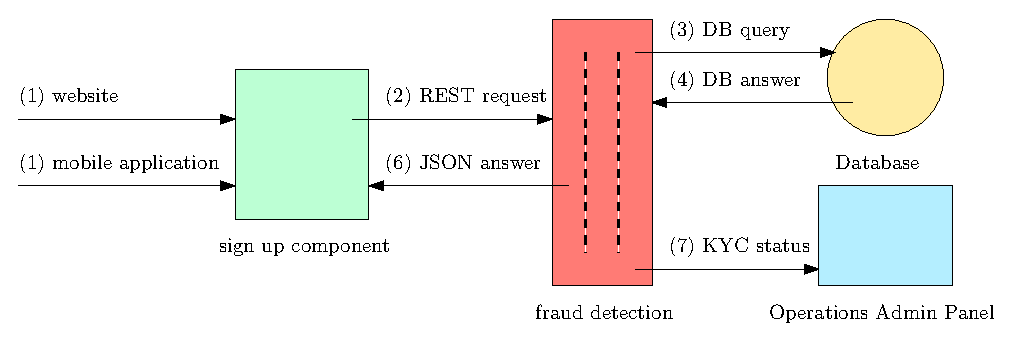
\includegraphics[width=\textwidth]{figures/fraud-arch2.eps}
    \end{center}
    \caption{The simplified architecture and strucutre of a PEP/HRA check request}
    \label{fig:fraud-arch}
\end{figure}

A request is triggered and answered with the following steps:

\begin{enumerate}
\item A new user signs up from one of the mobile apps or the website
\item The sign-up component sends a request for the new user to the fraud detection component
\item The component retrieves the necessary data from the database
\item The database delivers all matches based on first and last name
\item The Lookup algorithm is performed within the fraud detection component
\item The result is returned to the sign-up component with information of whether or not the user can continue the sign-up flow
\item The respective KYC actions and statuses are set in the database.
\end{enumerate}












%%%%%%%%%%%%%%%%%%%%%%%%%%%%%%%%%%%%%%%% CHAPTER Signature Recognition

\chapter{Fraud Detection \\Signature Verification}
\label{chp:signature-verification}

For centuries, being able to authenticate someone based on biometrics, has been important to identify each other, in order to conduct business and verify the authenticity or grant access to resources. In order to guarantee someone's identity, it has always been important to work towards more exact and more reliable means to measure someone's biometric properties and to match recorded properties against confirmed samples, while at the same time minimizing the chance of an erroneous accept or reject. The characteristic properties of a handwritten signature help to prove a signer's identity. A signature has four legal properties~\cite{Hanmandlu05}:

\begin{itemize}
\item \textbf{Authentication}: Signature verification allows to confirm a signer's identification
\item \textbf{Acceptance}: By signing a document, the writer conveys a willful intent and acceptance of the document's terms and contents
\item \textbf{Integrity}: By signing a document, the signer establishes the integrity of the signed document and that it has not been altered
\item \textbf{Non-repudiation}: The above three factors make it impossible for the signer to deny having signed the document
\end{itemize}

Signature verification is a particularly important biometric identification process since the signature is a widely accepted method for endorsing financial transactions~\cite{1227706}.
As the signature is recorded during the SAS and CAS authorization process, it makes sense for SumUp to use this information to improve the security of both authorization methods.

We present existing methods before describing the signature verification methods used in our work and the peculiarities for signature detection in mobile payments.
Traditionally, detection methods can be categorized as either global or local methods. We describe both approaches in Section \ref{sec:features} and Section \ref{sec:functions}. As a combination of feature- and function-based approaches has been providing better results than the individual techniques~\cite{fierrez2005line}, we combine both approaches in our method to verify signatures.


\section{Global Systems}
\label{sec:features}

Global systems, also called feature-based systems, are characterized by the fact that the feature vector consists of measurements that are based on the signature as a whole. The features are either analyzed as a whole or separately for each dimension. Often used global features include:

\begin{itemize}
\item Signature length
\item Total time to sign
\item Maximum and average velocity
\item Maximum acceleration
\item Total points recorded
\item Number of segments
\item Signature Height (H), Width (W) and W to H-Ratio
\item Number of points with positive $x$/$y$ velocity
\end{itemize}


A lot of research has been done in this area and the features can be simple measurements as those listed or more complicated characteristics obtained through techniques like the discrete Wavelet Transform \cite{ji2005signature}, the Hough Transform \cite{kaewkongka1999off}, horizontal and vertical projections \cite{fang2003off} or smoothness features \cite{fang2001offline}.

To compare two signatures with a global system, the features may be compared as
\begin{itemize}
\item absolute values
\item relative values in respect to another feature
\item averaged values over the whole signature or key parts of it
\item maximum or minimum values
\item values of the standard deviation
\end{itemize}

A benefit of comparing signatures based on global features is that they are generally faster to compute than local features and simple to store and compare because they can be represented by a number and don't require data structures.




\section{Local Systems}
\label{sec:functions}


Function-based systems, also called local systems, are characterized by the fact that the feature vector consists of measurements on individual points or clusters of points.
The most popular methods are Dynamic Time Warping and Hidden Markov Models. Often used local features include:

\begin{itemize}
\item Pressure
\item Horizontal ($x$) and vertical ($y$) position
\item Path tangent angle
\item Velocity and acceleration in a particular point
\item Log radius of curvature
\item Pen elevation and pen azimuth; In our case this data is not available as the signatures are written by finger
\end{itemize}

Typically, a function vector has fewer, or at most as many, dimensions as the signature vector. Matching two signatures requires finding an algorithm to match either
\begin{itemize}
\item two feature vectors
\item the vector of the test signature to a reference vector or model
\end{itemize}

Researchers have tried various techniques to match two feature vectors~\cite{PiyushShanker:2007:OSV:1274199.1274423}. Among these techniques are: Dynamic Time Warping \cite{Herbst98onan, citeulike:891512}, Hidden Markov Models \cite{Justino00anoff-line}, directional PDF \cite{drouhard_1996_pr}, stroke extraction \cite{1047809}, synthetic discriminant functions \cite{Wilkinson:91}, granulometric size distributions \cite{615447}, neural classifiers \cite{Bajaj19971}, wavelets\cite{Ramesh1999217}, grid features\cite{Qi19941621} and elastic matching\cite{citeulike:941886}.

% An overview over previous work was given in a paper by Guo et al.~\cite{Justino20051377}

Before trying one of these advanced techniques, one might try to compare two feature vectors in a simpler manner.
The simplest approach of comparing two feature vectors element by element is to use linear correlation \cite{Plamondon1989107} and calculate the distance between each pair.

This approach has two major drawbacks:
\begin{itemize}
\item It only works if the two vectors have equal length. As signatures always vary a bit, it is rarely the case that two signatures and thus the two feature vectors have equal length.
\item Even if the overall path of the signature is very similar, there often are parts that are distorted or additional in one of two signatures. Linear correlation is not able to account for local distortions and would thus create a bad score even if the beginning and end of the signature's path were a perfect match.
\end{itemize}

As both phenomena are very typical for signature verification, more advanced techniques were developed. Our work concentrates on Dynamic Time Warping and Hidden Markov Models as these two techniques have proven to be most successful --- especially when combined --- in previous work \cite{fierrez2005line, citeulike:885135, kashi1998hidden, PiyushShanker:2007:OSV:1274199.1274423,martens1996line}.

\newpage
\subsection{Dynamic Time Warping}


\begin{figure}
        \centering
        \begin{subfigure}[b]{0.30\textwidth}
                \centering
                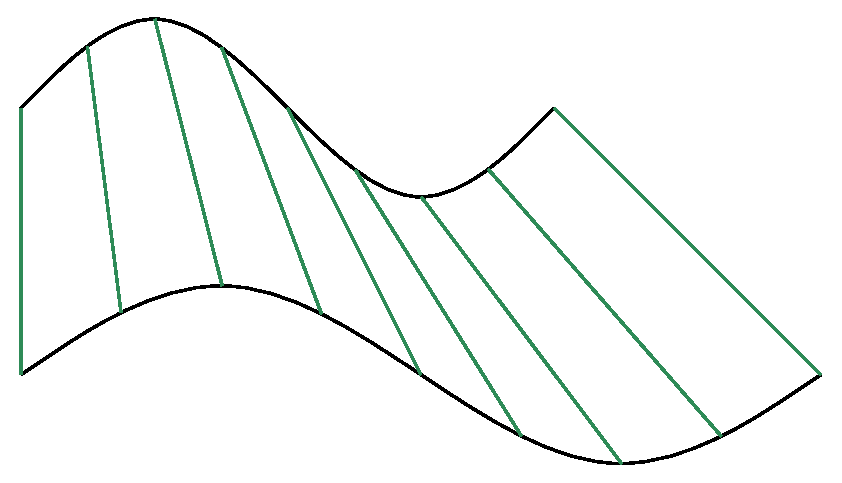
\includegraphics[width=\textwidth]{figures/dtw-stretch.eps}
                \caption{Scaling}
                \label{fig:hmm1}
        \end{subfigure}%
        \quad
        \begin{subfigure}[b]{0.30\textwidth}
                \centering
                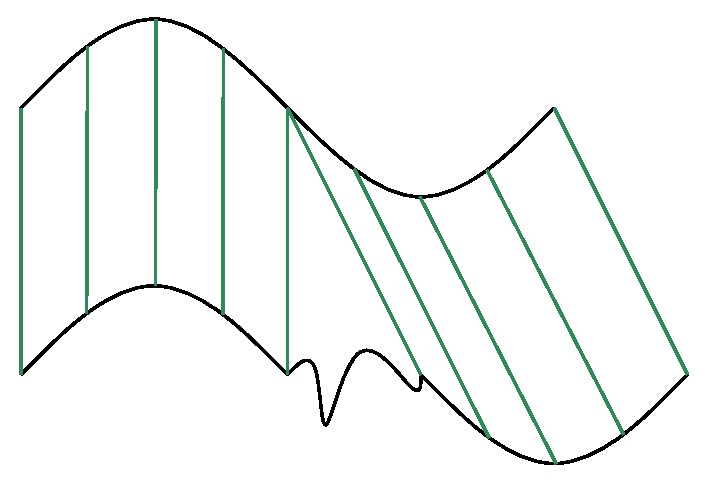
\includegraphics[width=\textwidth]{figures/dtw-distort.eps}
                \caption{Distortion}
                \label{fig:hmm1}
        \end{subfigure}%

        \caption{Two conceptual drawings show how DTW deals with the two main problems in signature recognition. The time series (a) is stretched but still matched thanks to DTW's ability to account for the scaling of segments or the signature as a whole. The drawing (b) is a representation of how DTW is still able to match two sequences even if one is distorted.}
        \label{fig:dtw-model}
\end{figure}



Dynamic Time Warping is a dynamic programming algorithm to measure the similarity between two time series which may vary in time or speed. This has been used for speech recognition and can also be used for signature detection to cope with  non-linear time distortions which can be seen in the signals because a signer does not always sign with the same speed. It has shown to be a much more robust distance measure than the Euclidean distance in a simple linear correlation~\cite{Keogh:2000:SUD:347090.347153, 1030918, 1227706} due to its ability to match similar shapes even if they are out of phase in the time axis.

Koegh et al.~\cite{Keogh:2002:EID:1287369.1287405} showed that the mean error rate average over 1000 runs for DTW was an order of magnitude lower than the error rate for the Euclidean distance. However, the DTW algorithm also took approximately 230 times longer to evaluate than the Euclidean distance.
It was applied to signatures in 1977 by Yasuhara and Oka \cite{yasuhara1977DTW} who concluded that it is a very useful approach for online real-time signature verification. Yasuhara and Oka used an adaption of the algorithm that was originally proposed by Sakoe and Chiba \cite{1163055} and improved the algorithm for the use on signature data.

As Figure \ref{fig:dtw-model} shows, DTW accounts for the two main difficulties when comparing two time series - stretching and distortion. This is of particular importance for our work, as we collect signatures on different devices with different sampling rates and even if a signer signs with the same speed but on two different devices, the two time series can significantly vary in length. Additionally, the different devices have different touchscreen sizes and surfaces and it is expected that people will not always complete the signature within the time due to different friction forces between finger and touchscreen and length of the signature path.

% \textbf{The concept} behind DTW is a dynamic algorithm that finds the shortest path in a matrix of the distance between each pair of dots. DTW can be used to compare two time series with each other and it is therefore inter


\textbf{Classification} is done by computing the DTW distance $dtw[s][t]$ between the model signature $s$ and a test signature $t$ which leads to a DTW score. If the score is below a certain threshold, we will consider the two signatures to match.

\textbf{Training} is done by computing the distance measure $dtw[n][m]$ for all signatures $n, m$ in the set of signatures for a certain user and selecting the signature $s$ with the smallest distance to all other signatures. While there are other techniques, which allow to build and train a signature model based on all the reference signatures, DTW can only compare two time series at once. Our strategy is to compute the DTW score for a test signature with each signature in the card holder's database and apply majority voting to decide if it's a forged or genuine signature.

\textbf{Algorithm}: We have two signature vectors $X,Y$ containing data for each point of the signatures:

$$X = x_1, x_2, ... , x_i, ... , x_I$$ $$Y = y_1, y_2, ..., y_j, ..., y_J$$

The distance between two vectors $x_i,x_j$ is defined as the 2-norm: $$d(i,j) = ||x_i - y_i||$$

We define a warping path $C$ as $$ C = c_1, c_2, ..., c_k, ..., c_K $$ where each element $c_k$ corresponds to a combination $(x_i, y_j)$.

The algorithm spans an $I \times J$ matrix $G$ between the two signature vectors. The matrix is initialized with $$g_1 = g(1,1) = d(1,1) \cdot w(1)$$ where $g_k$ is the accumulated distance after $k$ steps and $w(k)$ is a weighting function that has to be defined.
In each iteration, $g_k$ is computed as $$g_k = g(i,j) = \min\limits_{c_{k-1}} [g_{k-1}+d(c_k) \cdot w(k)]$$ until both Signatures $X,Y$ have been traversed.

The normalized distance of the two signatures is therefore: $$D(X,Y) = \frac{g_K}{\sum_{k=1}^K w(k)}$$ where $\sum w(k)$ compensates the effect of the length of the sequences.

The definitions of weighting factors $w_k$ defines the matching between the two signatures. The most common definition in literature is one where three types of transitions - deletion, match and insertion - are allowed. The resulting $g_k$ becomes:
$$g_k = g(i,j) = \min \left[\begin{array}{c}g(i,j-1) + d(i,j) \\g(i-1,j-1)+ 2 d(i,j) \\g(i-1,j) + d(i,j)\end{array}\right]$$

The first case corresponds to the case of insertion, the second to a match and the third to a deletion. If there is a match in each step, the path will go along the matrix' diagonal. Generally, if the path is close to the diagonal, the signatures are similar and the score is thus small.


\begin{figure}
        \centering
        \begin{subfigure}[b]{0.45\textwidth}
                \centering
                \includegraphics[width=\textwidth]{figures/dtw-graphic1.eps}
                % \caption{HMM1}
                \label{fig:hmm1}
        \end{subfigure}%
        \quad
        \begin{subfigure}[b]{0.45\textwidth}
                \centering
                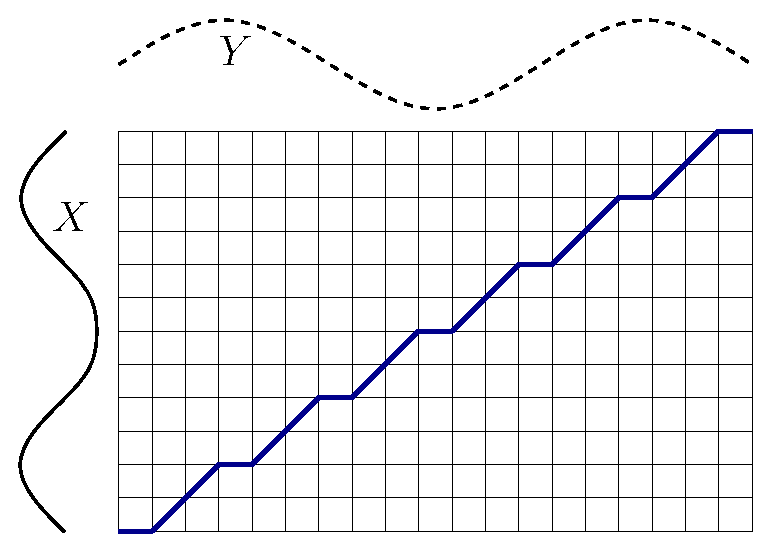
\includegraphics[width=\textwidth]{figures/dtw-graphic2.eps}
                % \caption{HMM1}
                \label{fig:hmm1}
        \end{subfigure}%

        \caption{Two slightly distoreted, strechted time series $X,Y$ can still be matched with the DTW algorithm as the diagonal warping path shows.}
        \label{fig:dtw-matrix}
\end{figure}



Even though the DTW algorithm has been outperformed by more powerful algorithms like HMMs or SVMs in speech detection, it remains very effective in signature detection as it deals well with small amounts of training data. This makes it an especially good fit for signature detection where the database of new users is usually sparse.

In general, DTW is known to have two drawbacks in signature verification:
\begin{itemize}
\item heavy computational load
\item warping of forgeries
\end{itemize}

DTW causes heavy computational load because it does not obey the triangular inequality and thus indexing a set of signatures takes a lot of time. It has complexity $\mathcal{O}(N^2)$ where $N$ is the signature length. As soon as the pool of signatures for a signer gets bigger, the computation costs rise because the test signature has to be compared to each of the signatures in the pool of confirmed signatures. Eamonn Keogh et al.~\cite{Keogh:2002:EID:1287369.1287405} presented a lower bounding method to index all samples without comparing each of them to each other. This is important when we analyze signatures in real time.

If a forgery is very close to the original, DTW might match it and not recognize it as different enough as it is one of the algorithm's strengths to account for scaling and minor distortions. This second drawback can be addressed by looking at how straight or bended the warping path is. A straight warping path indicates that a genuine signature is more likely whereas a curvy warping path indicates a forgery. Work on this has been done by Y. Sato et al.~\cite{Sato1982} but makes comparison between different signatures more difficult because it introduces another dimension and thus made computation harder and has hence not found widespread use.

% Hao Feng et al.~\cite{Feng:2003:OSV:961320.961331} proposed another extension of the DTW algorithm, called Extreme Points Warping (EPW). It proved to be more adaptive in the field of signature verification than DTW and reduces the computation time by a factor of 11.  Instead of warping the signature as a whole, they only warp so called Extreme Points that are characteristic to a signer's signature and match the curves between those points linearly.





\newpage
\subsection{Hidden Markov Models}
\label{sec-hmm}

A Hidden Markov Model is a stochastic process with an underlying Markov Model.
Unlike with classical Markov Models (MM), the states of a Hidden Markov Model cannot be directly observed. Only the symbols emitted from model's states may be observed. If the signature is interpreted as a succession of observed symbols, then we can, given an HMM, calculate the probability of each path through the states in the model. By training the HMM to match the signatures that are known to be genuine we can thus reconstruct a probability of the user matching.


\begin{figure}[tb]
    \begin{center}
        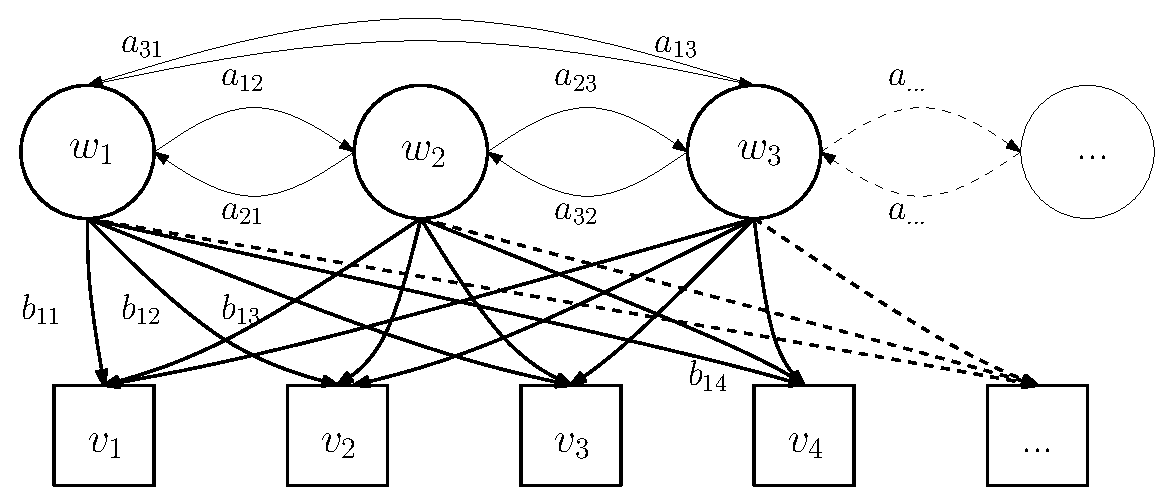
\includegraphics[width=\textwidth]{figures/hmm-general-model.eps}
    \end{center}
    \caption{General representation of an HMM with states $w_1, w_2, w_3, ...$, observations $v_1, v_2, v_3, ...$, the state transition probabilities $a_{ij}$ and the observation emission probabilities $b_{ij}$}
    \label{fig:hmm-general-model}
\end{figure}


An HMM, as illustrated in Figure \ref{fig:hmm-general-model}, is defined by:

\begin{itemize}
 \item $N$ hidden states $w_1, w_2, ..., w_N$
 \item the alphabet of $M$ of symbols $v_1, v_2, ...$
 \item the $N\times N$ transition matrix $A$, which fulfills
 $$\forall i,\qquad \sum_{j=1}^{N} a_{ij} = 1$$
 and whose elements are defined as
 $$a_{ij} \geq 0, \qquad a_{ij} = P(w_j(t+1)|w_i(t)), \qquad 1 \leq i,j \leq N$$

 \item the $N \times M$ emission matrix $B$, which fulfills
 $$\forall k,\qquad \sum_k b_j(k) = 1 $$
 and whose elements are defined as
 $$b_j(v(t)) = P(v(t)|w_j(t))$$

 \item the initial distribution $\pi$
\end{itemize}



The underlying Markov Model of an HMM is modeled depending on the application. The most common types are shown in Figure \ref{fig:markov-models}:
\begin{itemize}
\item Left-To-Right HMMs (LTR HMM) are characterized by the fact that from each state only the same state or a state more to the right can be reached. Once a state is left, it is never reached again. Depending on the application, no skipping of states (top left), skipping a single step (top right) or skipping an arbitrary number of states may be allowed (mid left). Which states can be reached from which other states is defined by the initial transition matrix. We define our transition matrix in Equation \ref{eq:hmm-transition-matrix} as an LTR model where no states can be skipped.
\item Parallel HMMs have parallel paths, only the states belonging to the same path can be reached once a path is chosen. They have similar properties to LTR Markov Models with the exception that there are multiple paths.
\item Ergodic HMMs are the most generic form of Markov Models where a transition is possible from any state to any other state or the same state. The transition matrix of an ergodic Markov Model has only non-zero elements.
\end{itemize}

In speech and signature recognition, a left-to-right Markov Model has proven to be a good choice. This can be interpreted as that a signer will never go back in his signature, which corresponds to the left-to-right analogy in the time series that corresponds to the signature.

\begin{figure}
        \centering
        \begin{subfigure}[b]{0.45\textwidth}
                \centering
                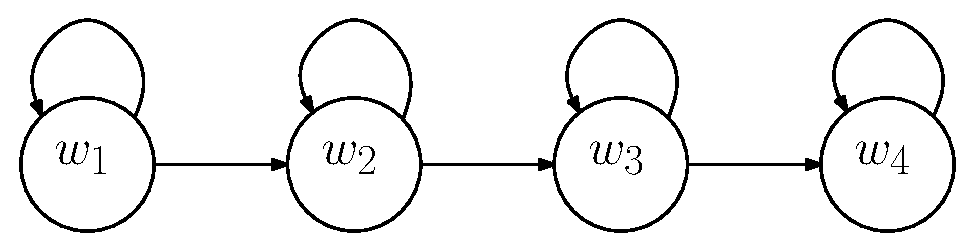
\includegraphics[width=\textwidth]{figures/hmm-ltr1.eps}
                \caption{}
                \label{fig:hmm1}
        \end{subfigure}%
        \quad
        \begin{subfigure}[b]{0.45\textwidth}
                \centering
                \includegraphics[width=\textwidth]{figures/hmm-ltr2.eps}
                \caption{}
                \label{fig:hmm1}
        \end{subfigure}%

        ~ %add desired spacing between images, e. g. ~, \quad, \qquad etc.
          %(or a blank line to force the subfigure onto a new line)
        \begin{subfigure}[b]{0.45\textwidth}
                \centering
                \includegraphics[width=\textwidth]{figures/hmm-ltr3.eps}
                \caption{}
                \label{fig:hmm1}
        \end{subfigure}%
        \quad
        \begin{subfigure}[b]{0.45\textwidth}
                \centering
                \includegraphics[width=\textwidth]{figures/hmm-ltr5.eps}
                \caption{}
                \label{fig:hmm1}
        \end{subfigure}%

        \begin{subfigure}[b]{0.45\textwidth}
                \centering
                \includegraphics[width=\textwidth]{figures/hmm-ltr4.eps}
                \caption{}
                \label{fig:hmm1}
        \end{subfigure}%



        \caption{Different types of HMMs: (a) LTR HMM where skipping of states is not allowed, (b) LRM with skipping of one step, (c) LRM with allowed skipping, (d) Parallel HMM, (e) Ergodic HMM}\label{fig:markov-models}
\end{figure}



While HMMs with a small set of states and observations perform bad because they are too simple, too many states and observations make the model computationally heavy and accuracy is reduced because of over-fitting.

The following three problems and their solutions is what makes HMMs so useful for real world applications:
\begin{enumerate}
\item \textbf{Evaluation}: Estimation of the optimal sequence of hidden states given the model parameters and observed data. This problem is solved by applying the Forward-Backward algorithm to the model.
\item \textbf{Decoding}: Calculation of the likelihood of the data given the model parameters and observed data. This is often solved with the Viterbi algorithm.
\item \textbf{Training}: Estimation of the model parameters given just the observed data. The Baum-Welch algorithm is used to estimate the model parameters.
\end{enumerate}

We are interested in the evaluation of an observed sequence to match a test signature to one of the signature models and we are interested in the training to train the signature models with the signatures we collect from a card holder. We follow previous authors who used the discretized angle between two points of a signature as the symbols. Based on those symbols, we train our model using the Baum-Welch algorithm. After training signature models, we calculate the likelihood of a signature belonging to a certain card holder by using the Forward-Backward algorithm to compare the signature to this card holder's signature model. A detailed description of all three problems and their solutions is given by Rabiner et al.~\cite{rabiner1989tutorial}.

In our case, we chose to work with an LTR HMM that does not allow skipping any states. This leads to a transition matrix $A$ of the form:
\begin{equation}
A = \left[\begin{array}{ccccc}a_{11} & a_{12} & 0 & \hdots & 0 \\0 & a_{22} & a_{23} & \cdots & 0 \\\vdots & \vdots & \vdots & \ddots & 0 \\0 & 0 & 0 & a_{(N-1)(N-1)} & a_{(N-1)N} \\0 & 0 & 0 & 0 & a_{NN}\end{array}\right]
\label{eq:hmm-transition-matrix}
\end{equation}


We also chose to work with a LTR HMM that does not skip any states and we chose $\pi$ such that the system starts in the first state:
$$\pi = \left[\begin{array}{cccc}1 & 0 & \cdots & 0\end{array}\right]$$


\textbf{The symbols} are calculated as the discretized angle between two points in a signature as illustrated in Figure \ref{fig:hmm-symbol-creation}. We use an alphabet of 4, 8 and 16 symbols in our experiment as described in Section \ref{sec:exp-reactive}.

\begin{figure}[tb]
    \begin{center}
        \includegraphics[width=0.6\textwidth]{figures/symbol-creation.eps}
    \end{center}
    \caption{Our symbols are defined as the discretized tangent angle. The left image represents a close up look of a signature and the points that define it. The drawing in the middle shows a zoomed version of the boxed segment and the tangent angle for the two points in this area. The right drawing shows the discretized $\gamma\prime$ for an alphabet of 8 symbols.}
    \label{fig:hmm-symbol-creation}
\end{figure}


\textbf{Evaluation: The Forward-Backward algorithm} is a recursive solution. Before looking at the algorithm in detail, we discuss a direct approach to evaluate the probability. A first approach to evaluate which model has produced a certain set of observations might be the following:
\begin{enumerate}
\item For all possible observation sequences, calculate the probability of going from the first to the last state while emitting that sequence
\item These probabilities sum up to the total probability $P(V^T)$
$$P(V^T) = \sum\limits_{r=1}^{r_\text{max}} P(V^T | w_r^T)P(w_r^T)$$
\item For all possible sequences in $w_r^T = w(1), w(2), ..., w(T)$ within $T$ time intervals we get
$$P(V^T) = \sum\limits_{r=1}^{r_\text{max}} \prod\limits_{t=1}^T  P(v(t) | w_(t)) P(w(t)|w(t-1))$$
\end{enumerate}
The problem with this approach is its time complexity of $\mathcal{O}(N^TT)$ which makes it unfeasible even for small values of N and T. E.g. for $N=5$ States and $T=100$ observations, there are on the order of $100 \cdot 5^{100} \approx 10^{72}$ computations.

Clearly, a more efficient method is required. Fortunately, there is The Forward-Backward algorithm is a recursive approach to approximate the solution.

\begin{enumerate}
\item We define the forward-backward variable which is the probability that a model is currently in state $i$ and has already produced the first $t$ elements of $V^T$
$$\alpha_i(t) = \begin{cases} \pi_i b_i(v(0)) & \mbox{if } t = 0 \\ \sum_{j=1}^N \alpha_j(t-1)a_{ij}b_j (v(t))& \mbox{if } t \ne 0 \end{cases}$$

\item For $t=0$ we initialize $a$
$$\alpha_i(0) = \pi_i b_i (v(0))$$

\item We compute $\alpha$ for all states $i$ at all times $t$
\item The total probability that a model $M$ generated the sequence $V^T$ results from the sum of all $\alpha_i(T)$

$$P(V^T|M) = \sum\limits_{i=1}^N \alpha_i(T)$$
\end{enumerate}

This algorithm is only of complexity $\mathcal{O}(N^2T)$ which results in our example to $5^2 \cdot 100 = 2500$ computations. Compared to the $10^72$, a saving of about 69 orders of magnitude --- as long as the number of states is reasonabily low.

In a similar way, we can consider a backward variable $\beta_i(t)$ defined as
$$\beta_i(t) = \begin{cases} 1 & \mbox{if } t = T \\ \sum_{j=1}^N \beta_j(t+1)a_{ij}b_j (v(t+1))& \mbox{if } t \ne T \end{cases}$$
The backward variable $\beta$ defines the probability of the partial observation sequence from $t+1$ to the end. In analogy to $\alpha$, we get the same computational complexity to compute $\beta$.


\textbf{Training: The Baum-Welch algorithm} is used to train signature model. The problem to adjust the model parameters $(A,B, \pi)$ to maximize the probability of the observed sequences is by far the most difficult of the three. There is no analytical way to solve for the model which maximizes the probability. We can, however, find a local maximum with an iterative procedure such as the Baaum-Welch algorithm.
The algorithm's output is the transition matrix $A$ that is most likely to generate the given sequence of observations. The following needs to be known about the model $M$ to start the algorithm:
\begin{itemize}
 \item the number of hidden states $N$
 \item one or more observations sequences $V_1, V_2, ...$
 \item the initial transition Matrix $A$, that defines the HMM's structure
 \item the initial distribution $\pi$
\end{itemize}


In order to get to an iterative solution, we proceed as follows:
\begin{enumerate}
\item We first define the probability of being in state $w_i$ at time $t-1$ and being in state $w_j$ at time $t$ as
$$
\xi_{ij} (t) = P(w_i(t), w_j(t+1)| V^T, M)
\\= \frac{\alpha_i(t)a_{ij}b_j(v(t+1))\beta_j(t+1)}{P(V^T|M)}
$$ $$\\= \frac{\alpha_i(t)a_{ij}b_j(v(t+1))\beta_j(t+1)}{\sum_k = 1^N \sum_l = 1^N \alpha_k(t)a_{kl}b_l(v(t+1))\beta_l(t+1)}
$$

\item By summing over $j$ we get the probability to be in state $w_i$ at time $t$ as

$$\gamma_i(t) = \sum\limits_{j=1}^N \xi_{ij}(t)$$



\item With that, we can calculate the number of transitions from $w_i$ to $w_j$ as
\begin{equation}
\sum\limits_{t=1}^{T-1} \xi_{ij}(t)
\label{eq-hmm2}
\end{equation}
and the expected number of transitions to any other state as
\begin{equation}
\sum\limits_{t=1}^{T-1} \gamma_{i}(t)
\label{eq-hmm3}
\end{equation}
\item And we get the expected number of times in one state from
\begin{equation}
\sum\limits_{t=1}^{T}\gamma_i(t)
\label{eq-hmm4}
\end{equation}

\item We get the expected number of times in state $w_i$ and observing symbol $k$ as
\begin{equation}
\sum_{t=1}^T \gamma_i(t)b_i(k)
\label{eq-hmm5}
\end{equation}


\item With that we can calculate:
\begin{itemize}
\item Expected Frequency (number of times) in state $w_i$ at time $t=0$ $\overline{\pi_i}= \gamma_i(0)$


\item Approximation of $a_{ij}$\\
$\overline{a_{ij}} = \frac{\mbox{(\ref{eq-hmm2})}}{\mbox{(\ref{eq-hmm3})}} = \frac{\sum_{t=1}^{T-1}\xi_{ij}(t)}{\sum_{t=1}^{T-1} \gamma_i(t)}$

\item Approximation of $b_{j}(k)$\\
$\overline{b_j(k)} = \frac{\mbox{(\ref{eq-hmm5})}}{\mbox{(\ref{eq-hmm4})}} = \frac{\sum_{t=1}^T \gamma_i(t)b_i(k)}{\sum_{t=1}^T \gamma_i(t)}$

\end{itemize}

\item Through repeated execution of this algorithm, we find the local maximum.

\end{enumerate}









\section{Challenges in Signature Detection Specific to Mobile Payments}

A lot of work has been done on signature detection on offline and online signatures. However, almost all work on dynamic signatures has been done on signatures that were written using a pen on a digital tablet or paper. In our case, signatures were captured on a wide range of different devices and with a user's finger instead of a pen.

\subsection{Signatures written with Finger}

Our experience shows that people are not used to write their signature with their finger and the first few times they sign, their signature differs a lot. However, after just 10-15 times, the signature's shape stabilizes.

This means that it will be a lot harder to detect signatures based on the first few signatures than on later signatures, once a user got used to signing with her finger.
We notice that a card holder's signature characteristics stabilize once used to signing with a finger. We therefore prefer most recent signatures to older ones when we apply the algorithms implemented in Chapter \ref{sec:exp-reactive}

\subsection{Sparse Initial Dataset}

Although SumUp is live in over ten countries as of April 2013, it is still only used in a relatively small set of locations and we are therefore unlikely to gather a lot of data about a single user until the concept becomes more often deployed and used.

This means that we have to try and find a solution that works reasonably well with a small amount of initial data per user. The problem persists even after this initial phase as new people will continue to join and always start with an empty set of signatures. We therefore test the algorithms developed in Chapter \ref{sec:exp-reactive} not only on the whole database for a card holder but also on small subsets.


\subsection{Device and Software Fragmentation}

Unlike signatures captured on a digital tablet, our database of signatures is captured on a variety of devices with different properties. There are various factors that have an influence on the digital representation of the signature:

\begin{itemize}
\item Different Manufacturers: Both, iOS and Android devices use a variety of manufacturers for their handsets and the built-in touch screens.
\item Screen Size: the screen diagonal of current smartphones typically ranges between three and six inches, those of tablets typically range between seven and eleven inches. A consequence is that the user might not only sign slightly differently but also that the signature will consist of more data points and it will take users a longer to sign on a larger screen.
\end{itemize}

We normalize the signature data before applying the algorithms in Chapter \ref{sec:exp-reactive} to account for these device-specific differences.






\section{Feedback Loop}

Due to the mentioned challenges, our systems are likely not to perform as well as the same systems on traditional signatures captured by pen on a digital tablet. We are likely to get results with a higher Equal Error Rate (EER) which would hurt SumUp's business since we declined transactions because of false positive matches.

To eliminate the risk of blocking transactions because of a false positive match, we propose to use a feedback loop along with our signature verification system.

A simple approach to use signature verification is shown in Figure \ref{fig:fb-loop1}:
\begin{itemize}
\item The mobile device sends the signature data along with a transaction request to SumUp's backend
\item The signature data is analyzed and compared to this user's signature model to generate a score
\item The score is compared to a threshold for this user's signature model and the signature is classified as genuine or forged
\item Based on the outcome the signature is either accepted or declined
\end{itemize}

This means that a user has no way of processing a card transaction if the signature does not pass the threshold that is generated based on his previous signatures. To overcome this problem, we suggest to use a feedback loop as shown in \ref{fig:fb-loop2}. Instead of declining a transaction, a request is sent to the merchant to confirm the identity of the card holder. If the merchant is able to confirm the card holder's identity, the transaction is processed. If the merchant is unable to confirm the identity, the card holder is reported as he is most probably a stolen or copied card.

This approach has several benefits:
\begin{itemize}
\item A signature evolves over time. With a feedback loop, the system can adapt over time to eveolving signatures.
\item The feedback loop helps to train the algorithm as we get very specific feedback on the false negative matches and can correct the algorithm without extra testing in field groups.
\end{itemize}

\begin{figure}
        \centering
        \begin{subfigure}[b]{\textwidth}
                \centering
                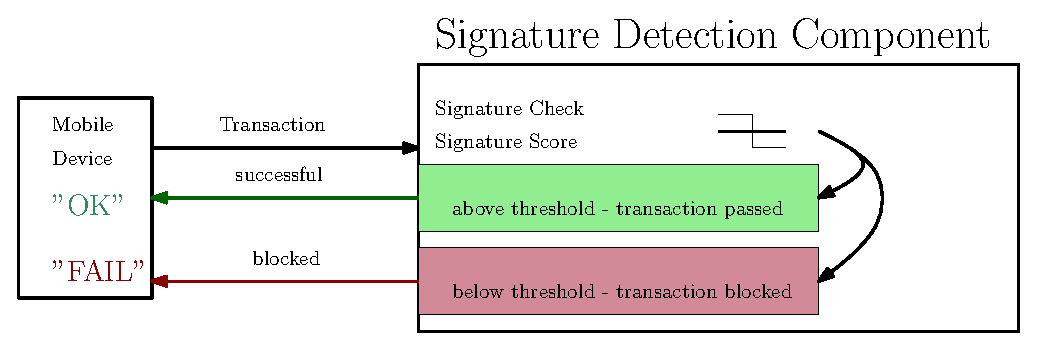
\includegraphics[width=1\textwidth]{figures/fb-loop1.eps}
                \caption{Simplified illustration of processing a transaction without the feedback loop. When the transaction object is received, the signature is extracted and analyzed. The score is compared with a threshold and if too low, the transaction is blocked. In case of a false positive match, this transaction is lost which we need to avoid.}
                \label{fig:fb-loop1}
        \end{subfigure}%

        \begin{subfigure}[b]{\textwidth}
                \centering
                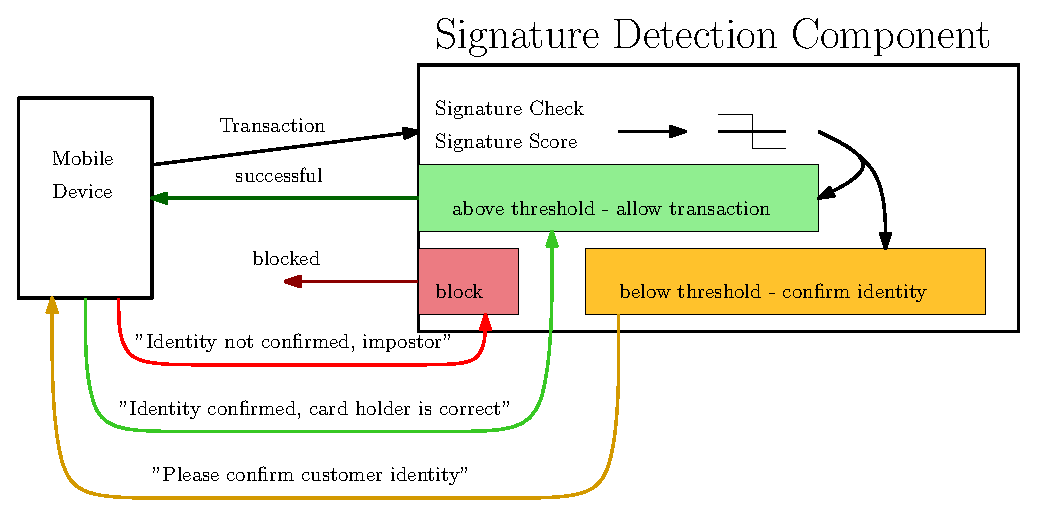
\includegraphics[width=1\textwidth]{figures/fb-loop2.eps}
                \caption{Simplified illustration of processing a transaction with the feedback loop. If the signature check does not reach the acceptance level, a request is sent to the merchant to confirm the card holder's signature. After a positive confirmation, the transaction is processed and otherwised blocked.}
                \label{fig:fb-loop2}
        \end{subfigure}%
        \caption{A traditional signature detection system based on a threshold (a) and the extended system that includes a feedback loop (b) }
        \label{fig:feedback-loop}
\end{figure}









%%%%%%%%%%%%%%%%%%%%%%%%%%%%%%%%%%%%%%%% CHAPTER EXPERIMENTS
\chapter{Implementation and Evaluation}
\label{chp:experiments}


Our work on fraud prevention was implemented and released to SumUp's production environment. Section \ref{sec:exp-preventive} describes the implementation's setup and performance. We show how the new check's performance has affected the work of SumUp's operations team and to which extent we were able to reduce the amount of false positives.

We discuss our fraud detection system in Section \ref{sec:exp-reactive}. We introduced the database used for our experiments and give a detailed description of the performance of the separate algorithms used. We also discuss the technical feasibility of each approach and the fusion of all three scores.


\section{Preventive Fraud Detection}
\label{sec:exp-preventive}

The algorithms described in Listing \ref{lst:world-check-parse} and Listing \ref{lst:world-check-lookup} were implemented in a Ruby Sinatra application with a REST interface and the application was deployed to production six weeks prior to the submission of this report.

\subsection{Setup}

The full World-Check PEP/HAR database was parsed in a testing environment using the algorithm in Listing \ref{lst:world-check-parse} and the parsed data was copied into the production database. The daily, incremental updates are downloaded from the World-Check servers into the production environment and are directly parsed into the production database.

The PEP/HRA check is performed automatically or manually in at least three occasions:
\begin{itemize}
\item \textbf{Automatically} for each new user during sign-up
\item \textbf{Automatically} for each existing user at the end of each week to re-check each account after incorporating the incremental updates of that week
\item \textbf{Manually} from the SumUp Operations Admin Panel (SOAP) via a button
\end{itemize}

Each request is triggered via a POST request. Depending on the user type to be checked, the body of the request changes. Table \ref{tbl:har-pep-requests} lists the different request types.

\begin{table}[tb]
    \begin{center}
        \begin{tabular}{p{1.75cm}|p{3cm}p{7cm}}
        \hline
        \textbf{Method} & \textbf{Path} & \textbf{Parameter} \\
        \hline
        POST & /person/check & \{"params": \{"user\_id": "1"\}\} \\ \hdashline[0.5pt/3pt]
        POST & /person/check & \{"params": \{"business\_owner\_id": "1"\}\} \\ \hdashline[0.5pt/3pt]
        POST & /person/check & \{"params": \{"business\_officer\_id": "1"\}\} \\
        \hline
        \end{tabular}
    \end{center}
    \caption{The requests received by the PEP/HAR component}
    \label{tbl:har-pep-requests}
\end{table}

\subsection{Results}

The new component was released to production at beginning of calendar week 10 on March 4th, 2013. At the same time, the old check was discontinued. Every new user since then was automatically checked during the sign-up process. In addition to that, Business Officers and Owners were checked manually through SOAP by the Operations Team. The following data refers to checks during the sign-up process and excludes data from weekly re-checks or manual requests.

As SumUp is still growing rapidly, all numbers were normalized in respect to 1000 new sign-ups per week. The number of manual work by the operations team could be greatly reduced thanks to a much lower rate of false positives and therefore less matches which have to be manually confirmed or rejected. Figure \ref{fig:pep-hra-charts} shows how the number of matches declined in calendar week 10 after the release of the new component.
The high amount of false positive matches which had to be checked by the operations team caused a backlog which is clearly visible by the shifted red curve in Figure \ref{fig:pep-hra-charts}. Due to the high amount of manual work that was required to reject or approve a match, the false positives were often only rejected --- and thereby marked as a false positive match  --- one or two week after the initial match.

Typically, about 50 to 100 matches were generated per 1000 new users with the old component. Almost all of those were false positives and therefore caused unnecessary manual work. With the new component, we were able to drastically reduce the amount of manual work required. After introduction of the new check to the system, the typical amount of matches per 1000 new sign-ups after the release of the new component declined to below ten and the amount of false positive matches was less than two. The higher number of false positive matches in week 13-10 was influenced by the backlog of previous weeks but it quickly stabilized from week 13-11 ongoing as shown in Table \ref{tbl:hra-pep-results}. The peak in calendar week 14 was caused by a system migration in the course of which a lot of accounts were checked again. However, as these accounts had been previously rejected, they did not cause any additional manual work.

The numbers in Table \ref{tbl:hra-pep-results} show that the number of false positive matches could be reduced from 50-80 per 1000 sign-ups to less than two which corresponds to a reduction of over 96 percent.

SumUp's operations team reports the reduction had a significant impact on their work. The amount of work hours per week in this area has declined from more than seven to less than one hour on average as shown in Table \ref{tbl:man-hours}. These are absolute numbers and do not account for the continued exponential growth of new sign-ups. The amount of work hours in this area has been almost doubling every month before the release of the new component in march.

\begin{table}[tb]
    \begin{center}
        \begin{tabular}{cc|c|cc}
        & Week  & Matches [per 1000 sign-ups]   & False Positive Matches \\ \cline{2-5}
\multirow{6}{*}{
\begin{sideways}
after release
\end{sideways}
}  & 13-15 & 3,29      & 1,39                \\ \cdashline{2-5}[0.5pt/3pt]
       & 13-14 & 25,36     & 1,40            \\ \cdashline{2-5}[0.5pt/3pt]
       & 13-13 & 1,77      & 0,98            \\ \cdashline{2-5}[0.5pt/3pt]
       & 13-12 & 2,84      & 0,95            \\ \cdashline{2-5}[0.5pt/3pt]
       & 13.11 & 2,20      & 2,42            \\ \cdashline{2-5}[0.5pt/3pt]
       & 13-10 & 2,64      & 6,71            \\ \cline{2-5}\cline{2-5}
\multirow{6}{*}{
\begin{sideways}
before release
\end{sideways}
       }  & 13-09 & 64,33     & 58,91          \\ \cdashline{2-5}[0.5pt/3pt]
       & 13-08 & 60,71     & 53,99             \\ \cdashline{2-5}[0.5pt/3pt]
       & 13-07 & 55,89     & 55,89             \\ \cdashline{2-5}[0.5pt/3pt]
       & 13-06 & 77,83     & 77,83             \\ \cdashline{2-5}[0.5pt/3pt]
       & 13-05 & 65,10     & 36,86             \\ \cdashline{2-5}[0.5pt/3pt]
       & 13-04 & 71,00     & 68,73             \\ \cline{2-5}
        \end{tabular}
    \end{center}
    \caption{The matches and false postivies generated by the fraud prevention component before and after release of the new component.}
    \label{tbl:hra-pep-results}
\end{table}

\begin{figure}
        \centering
        \begin{subfigure}[b]{\textwidth}
                \centering
                \includegraphics[width=\textwidth]{figures/chart_total.png}
                % \caption{HMM1}
                \label{fig:chart-total}
        \end{subfigure}%

        \begin{subfigure}[b]{\textwidth}
                \centering
                \includegraphics[width=\textwidth]{figures/chart_pep.png}
                % \caption{HMM1}
                \label{fig:chart-pep}
        \end{subfigure}%

        ~ %add desired spacing between images, e. g. ~, \quad, \qquad etc.
          %(or a blank line to force the subfigure onto a new line)
        \begin{subfigure}[b]{\textwidth}
                \centering
                \includegraphics[width=\textwidth]{figures/chart_har.png}
                % \caption{HMM1}
                \label{fig:chart-har}
        \end{subfigure}%

        \caption{Evolution of the number of matches generated by the automatic PEP/HRA check. The top graph shows the evolution of the overall matches and false positives and the bottom and bottom graph the evolution for PEP and HRA separately. The new check was released to production in week 13-10 which is clearly visible as both numbers decline. The shifted false positives indicate the backlog of records that had to manually confirmed or rejected.}
        \label{fig:pep-hra-charts}
\end{figure}



\begin{table}[tb]
    \begin{center}
        \begin{tabular}{c|c|c}Month & Matches (absolute numbers) & Man Hours \\ \hline
        December & 283 & 10 hours \\ \hdashline[0.5pt/3pt]
        January & 463 & 16 hours  \\ \hdashline[0.5pt/3pt]
        February & 853 & 29 hours \\ \hline
        March & 125 & 4 hours \\ \hdashline[0.5pt/3pt]
        April 1st - 14th & 9 & 0.3 hours \\ \hline
        \end{tabular}
    \end{center}
    \caption{The absolute numbers of matches and man hours caused by matches and false positives. The new component was released at the beginning of march and the impact on the number of work hours is significant.}
    \label{tbl:man-hours}
\end{table}


















\section{Reactive Fraud Detection}
\label{sec:exp-reactive}

\subsection{Database}

As there is no publicly available database of signatures written by finger and captured by a smartphone's touch screen, we created a database for the purpose of this research.
Between eight and 80 Signatures per person were collected from ten people on four different days on four different devices. This approximates the reality in terms of how many signatures SumUp has available per card holder and the devices they were collected with. In total, a set of 487 signatures was collected.
The devices used to collect the signatures are listed in Table \ref{tbl:signatures-devices} and were all used equally often.

\begin{table}[tb]
    \begin{center}
        \begin{tabular}{p{1.75cm}|p{2cm}p{2cm}p{2cm}p{2cm}}
        \hline

        \hline
        \textbf{Device} & \textbf{Software Version} & \textbf{Screen Size [cm]} & \textbf{Screen Resolution [px]} & \textbf{Pixel Density [ppi]} \\
        \hline
        Apple iPhone 4s & iOS 6.1.2 & 8.9 & 640x960 & 326 \\
        \hdashline[0.5pt/3pt]
        Apple iPhone 5 & iOS 6.1.2 & 10 & 640x1136 & 326 \\
        \hdashline[0.5pt/3pt]
        Samsung Galaxy Note II & Android 4.1.1 & 14.1 & 720x1280 & 267 \\
        \hdashline[0.5pt/3pt]
        Apple iPad mini & iOS 6.1.2 & 20 & 768x1024 & 163\\
        \hline
        \end{tabular}
    \end{center}
    \caption{The four devices used to collect signatures, ordered by screen size}
    \label{tbl:signatures-devices}
\end{table}

We also collected three forgeries for each person. The forgeries were created by two untrained persons and are of the following types:

\begin{itemize}
\item \textbf{Spontaneous Forgery $\mathcal{F}_1$}: A random signature from one card holder's  signature set was shown to the impostor during five seconds. The impostor was allowed to start the forgery after the five seconds when he had no access to the signature anymore.
\item \textbf{Sample Forgery $\mathcal{F}_2$}: A random signature from one card holder's signature set was shown to the impostor for an indefinite amount of time and the impostor was able to look at the signature while forging the signature.
\item \textbf{Knowledgeable Forgery $\mathcal{F}_3$}: The impostor had unlimited access to a card holder's full signature set while creating the forgery.
\end{itemize}


For each technique described in Section \ref{sec:global-features} - \ref{sec:hidden-markov-models}, we gathered statistics about two use cases:
\begin{itemize}
\item \textbf{Classification of signatures}: This approach's goal is to measure how well the algorithm performs in connecting a signature with its card holder. In this part we run the ground truth against itself to train the algorithm and adjust its parameters.
\item \textbf{Detection of forgeries}: Using the previously obtained parameters, we run the algorithm against the database of forgeries to see which of the forgeries are correctly detected. This corresponds to SumUp's use case of our fraud detection work.
\end{itemize}

All experiments were conducted on a current Mac OS/Unix system and run within a single thread. It is expected that the time needed to compute results could be reduced by using parallel execution of the algorithms. SumUp's server hardware exceeds this Mac OS/Unix system's computation power. We can assume that the execution times are  even shorter on the production system.

\subsection{Pre-Alignment and Normalization}

In order to compare the signatures, we normalized some of the properties before comparing the signatures. To account for the fact that the signatures were collected on devices with specific characteristics, the following parameters were normalized:

\begin{itemize}
\item \textbf{Sampling rate}: Because we collected the signatures on touchscreen devices with event-based sampling, we recorded very different sampling rates between devices but also within the data for one signature. Typically, signatures collected on iOS devices were originally sampled at a rate of 40 Hz and signatures collected on the Android device at 60 Hz. In order to compare signatures, we normalize the sampling rate to 20 Hz for all signatures which equates about half of the typical sampling rate of a signature collected on an iPhone 4s.
\item \textbf{Size and length}: The different screen sizes and pixel densities caused different height, width and length properties. In order to compare the signatures, we normalized the signatures height and width to fit within a 200 pixel by 300 pixel rectangle. The width-to-height ratio was recorded before the normalization as it is used as a global feature in Section \ref{sec:global-features}.
\item \textbf{Time}: As bigger screen sizes also means longer distances to draw a signature, we adjusted the timestamps when we normalized the size of a signature. We referred to the normalized value when we used time in Section \ref{sec:global-features}.
\end{itemize}





\subsection{Global Features}
\label{sec:global-features}

Our implementation of a signature verification system based on global features uses a subset of the proposed features in Section \ref{sec:features}. Our system relies on the following features:

\begin{itemize}
\item Signature length $l$ in pixels
\item Total time to sign  $t$ in milliseconds
\item Maximum and average velocity $v_\text{max}, \bar{v}$
\item Maximum acceleration $a_\text{max}$
\item Number of segments $n$
\item Width to height ration $r$
\end{itemize}

Other proposed features, e.g.\ the total number of points recorded, are irrelevant for our experiments as we normalize those features in order to compare signatures captured on different devices.
Figure \ref{fig:global-features} shows our results for each card holder's signature set. We list the minimum (Table \ref{tbl:global-features-results-min}), average (Table \ref{tbl:global-features-results-avg}) and maximum (Table \ref{tbl:global-features-results-max}) value for each feature and card holder.

\begin{figure}
    \centering
    \begin{subfigure}[b]{\textwidth}
            \centering
            \small
            \begin{tabular}{c|c|c|c|c|c|c|c}
            \hline
            \textbf{P} & $l$ & $t$ & $v_\text{max}$ & $\bar{v}$ & $a_\text{max}$ & $n$ & $r$\\
            \hline
            0 & 1316.81 & 1640.0 & 2.27 & 0.8 & 1.11 & 2.0 & 0.0 \\ \hdashline[0.5pt/3pt]
            1 & 827.09 & 1373.0 & 1.5 & 0.6 & 0.58 & 2.0 & 1.0 \\ \hdashline[0.5pt/3pt]
            2 & 839.37 & 1445.0 & 1.71 & 0.58 & 0.7 & 2.0 & 2.0 \\ \hdashline[0.5pt/3pt]
            3 & 1434.08 & 2250.0 & 2.22 & 0.64 & 1.49 & 3.0 & 2.0 \\ \hdashline[0.5pt/3pt]
            4 & 669.82 & 1122.0 & 1.79 & 0.6 & 0.49 & 1.0 & 2.0 \\ \hdashline[0.5pt/3pt]
            5 & 924.78 & 1856.0 & 1.14 & 0.5 & 0.64 & 2.0 & 2.0 \\ \hdashline[0.5pt/3pt]
            6 & 1281.41 & 1399.0 & 2.49 & 0.92 & 1.53 & 2.0 & 1.0 \\ \hdashline[0.5pt/3pt]
            7 & 843.17 & 1424.0 & 1.13 & 0.59 & 0.48 & 2.0 & 1.0 \\ \hdashline[0.5pt/3pt]
            8 & 639.14 & 1209.0 & 1.7 & 0.53 & 0.73 & 1.0 & 1.0 \\ \hdashline[0.5pt/3pt]
            9 & 1299.5 & 5467.0 & 0.79 & 0.24 & 0.41 & 4.0 & 1.0 \\
            \hline
            \end{tabular}
            \caption{The minimum values for each signature set and all global features}
            \label{tbl:global-features-results-min}
    \end{subfigure}%

    \begin{subfigure}[b]{\textwidth}
            \centering
            \small
            \begin{tabular}{c|c|c|c|c|c|c|c}
            \hline
            \textbf{P} & $l$ & $t$ & $v_\text{max}$ & $\bar{v}$ & $a_\text{max}$ & $n$ & $r$\\
            \hline
            0 & 1701.69 & 1942.75 & 15.5 & 0.88 & 16.93 & 2.13 & 0.5 \\ \hdashline[0.5pt/3pt]
            1 & 1235.27 & 1773.95 & 11.24 & 0.7 & 13.36 & 2.0 & 1.93 \\ \hdashline[0.5pt/3pt]
            2 & 1206.72 & 1762.06 & 10.22 & 0.68 & 18.96 & 3.11 & 2.33 \\ \hdashline[0.5pt/3pt]
            3 & 2565.76 & 3217.96 & 17.62 & 0.8 & 27.72 & 5.58 & 2.42 \\ \hdashline[0.5pt/3pt]
            4 & 1104.21 & 1588.11 & 8.1 & 0.7 & 9.58 & 3.43 & 2.81 \\ \hdashline[0.5pt/3pt]
            5 & 1308.19 & 3047.47 & 5.23 & 0.43 & 8.25 & 8.0 & 2.3 \\ \hdashline[0.5pt/3pt]
            6 & 2480.3 & 2102.87 & 13.71 & 1.18 & 16.89 & 3.87 & 2.04 \\ \hdashline[0.5pt/3pt]
            7 & 1260.28 & 2194.41 & 6.79 & 0.57 & 9.41 & 2.64 & 2.07 \\ \hdashline[0.5pt/3pt]
            8 & 1311.1 & 1574.98 & 11.18 & 0.83 & 15.12 & 2.6 & 1.47 \\ \hdashline[0.5pt/3pt]
            9 & 2047.7 & 6953.81 & 3.95 & 0.29 & 5.04 & 12.19 & 2.4 \\
            \hline
            \end{tabular}
            \caption{The average values for each signature set and all global features}
            \label{tbl:global-features-results-avg}
    \end{subfigure}%

    ~ %add desired spacing between images, e. g. ~, \quad, \qquad etc.
      %(or a blank line to force the subfigure onto a new line)
    \begin{subfigure}[b]{\textwidth}
            \centering
            \small
            \begin{tabular}{c|c|c|c|c|c|c|c}
            \hline
            \textbf{P} & $l$ & $t$ & $v_\text{max}$ & $\bar{v}$ & $a_\text{max}$ & $n$ & $r$\\
            \hline
            0 & 2571.75 & 2282.0 & 54.42 & 1.13 & 73.35 & 3.0 & 1.0 \\ \hdashline[0.5pt/3pt]
            1 & 2048.9 & 2957.0 & 82.49 & 0.69 & 139.0 & 2.0 & 3.0 \\ \hdashline[0.5pt/3pt]
            2 & 2069.97 & 2117.0 & 52.35 & 0.98 & 105.95 & 5.0 & 3.0 \\ \hdashline[0.5pt/3pt]
            3 & 4673.42 & 9370.0 & 104.48 & 0.5 & 180.54 & 8.0 & 4.0 \\ \hdashline[0.5pt/3pt]
            4 & 2041.9 & 2914.0 & 63.79 & 0.7 & 99.93 & 5.0 & 4.0 \\ \hdashline[0.5pt/3pt]
            5 & 2425.82 & 4694.0 & 41.11 & 0.52 & 48.09 & 11.0 & 4.0 \\ \hdashline[0.5pt/3pt]
            6 & 4388.68 & 3633.0 & 75.89 & 1.21 & 134.83 & 5.0 & 3.0 \\ \hdashline[0.5pt/3pt]
            7 & 1958.88 & 4349.0 & 65.51 & 0.45 & 92.97 & 8.0 & 3.0 \\ \hdashline[0.5pt/3pt]
            8 & 2146.82 & 2749.0 & 65.46 & 0.78 & 112.3 & 4.0 & 2.0 \\ \hdashline[0.5pt/3pt]
            9 & 3428.25 & 8083.0 & 20.12 & 0.42 & 33.69 & 17.0 & 9.0 \\
            \hline
            \end{tabular}
            \caption{The maximum values for each signature set and all global features}
            \label{tbl:global-features-results-max}
    \end{subfigure}%

    \caption{The minimum, average and maximum values we obtained for all global features for each subject's set of signatures.}
    \label{fig:global-features}
\end{figure}


\textbf{Similarity score $S_{GF}$}\\
We use our knowledge about the minimum, average and maximum value for each of the signature sets to create a similarity score.
For a test signature $s_t$, we compute the seven global features. For each feature of the test signature that lies within the card holder's maximum and minimum values, we assign a 1 in the score vector $G$. If the test value does not lie within this window, we assign a 0.
$$G = [g_l, g_t, g_{v_\text{max}}, g_{\bar{v}}, g_{a_\text{max}}, g_n, g_r], g \in \{0,1\}$$

We assume that not all of the global features are of the same significance. We therefore define a  weighting vector $$W = [w_l, w_t, w_{v_\text{max}}, w_{\bar{v}}, w_{a_\text{max}}, w_n, w_r]$$

Our similarity score is calculated as the cross product of the score vector $G$ and the weighting vector $W$:
$$S_{GF} = G \times W$$

As every signature added to the database possibly enlarges the window between a card holder's minimum and maximum value for each feature, a sliding window should be used for larger datasets. As we were are working with less than 50 signatures per card holder, we did not implement a sliding window mechanism as part of our research.

\textbf{Fitness function $\mathbb{F}_{GF}$}\\
In order to find the best performing weighting vector $W$, we run each signature against each of the ten signature models and minimize the number of false positive matches. A signature model is defined by the minimum/maximum range for each feature.

By definition, all signatures will score a perfect score at least once. The fitness function $\mathbb{F}_{GF}$ tries to get as close to that number as possible. Starting with the weighting vector $W = [0, 0, 0, 0, 0, 0, 0]$, the first result corresponds to the total number of signatures used for this experiment. By exploring all possible $W$ for $w \in {0,1,2}$, the algorithm finds the $W$ for which the least elements the highest similarity score  $S_{GF}$ at the same time.

The fitness function for global features $\mathbb{F}_{GF}$ is defined in pseudo code in Listing \ref{lst:global-features-fitness-function}.

\begin{figure}
\begin{lstlisting}[caption={The fitness function for global features tries to reduce the number of signatures with the hightes possible score for a given weighting vector $W$},label={lst:global-features-fitness-function}]

until fitness == #signatures_in_groundtruth

    fitness = calculate_globabl_features w

    if fitness < previous_fitness
        save w
    end

    permutate w
end
\end{lstlisting}
\end{figure}

\textbf{Classification of Signatures}\\
We defined the start vecor $W = [0,0,0,0,0,0,0]$ and let the fitness function permutate the vector until a local minimum was found. The local minimum was reached for $$W = [w_l, w_t, w_{v_\text{max}}, w_{\bar{v}}, w_{a_\text{max}}, w_n, w_r] = [0, 1, 0, 1, 0, 1, 1]$$


We used a subset of 278 signatures for this experiment. The local minimum was reached at 755 signatures that scored the a similarity score $S_{GF} =4$ for the same $W$. This includes 478 signatures more than the global minimum.
From $W$ we conclude that time $t$, average velocity $\bar{v}$, the number of segments $n$ and the width-to-height ratio $r$ are the important global features and should be used to compare signatures and detect forgeries.

When we extend the fitness function to include the two groups with the highest occurrences, we get 840 signatures in the top tier and the weighting vector $W'$ which confirms the importance of the same features.
$$W' = [w_l, w_t, w_{v_\text{max}}, w_{\bar{v}}, w_{a_\text{max}}, w_n, w_r] = [0, 2, 0, 2, 0, 2, 1]$$



\textbf{Detection of forgeries}\\
We used the previously found weighting vector $W$ to test the robustness of this approach against forgeries. We set $$W = [0, 1, 0, 1, 0, 1, 1]$$
and run all forgeries against the previously trained signature models, which are defined by the minimum and maximum values.

For each forgery, we compute the value of each of the four important global features, $t, \bar{v}, n$ and $r$. We compare the generated value to the the bounds for that feature for each person. A match requires that the test value lies within the reference minimum and maximum for all four features. The results are shown in Figure \ref{fig:global-features-forgeries}. The tables first lists the minimum and maximum for each feature and card holder, the value found for the forgery and whether the signature was correctly rejected as a forgery or accepted (a false positive match).

All but one forgeries were correctly rejected as forgeries. We notice that most of the forgeries were rejected mostly because the impostor took too long to sign ($t$ too high) or because he did not sign fast enough ($\bar{v}$ too little). We achieve an error rate of 3.33 percent with this system.

\textbf{Real time feasibility}\\
Computing the features for a signature and comparing them to the previously computed minimum and maximum values takes less than one hundredth of a second. By using a sliding window, the computational complexity of computing the minimum and maximum values is guaranteed to have an upper bound even if the total amount of signatures for a card holder may grow to very large. We conclude that this approach is feasible for real time application.

\begin{figure}
    \centering
    \begin{subfigure}[b]{\textwidth}
            \centering
            \tabcolsep 4pt
            \small
            \begin{tabular}{c|cccc||cccc||c}
            \hline
            \textbf{P} & $t_r$ & $\bar{v}_r$ & $n_r$ & $r_r$ & $t_f$ & $\bar{v}_f$ & $n_f$ & $r_f$ & Hit \\
            \hline
            0 & [1640.0, 2282.0] & [0.8, 1.13] & [2.0, 3.0] & [0.0,1.0] & 13782.0 & 0.14 & 2.0 & 2.0 & \xmark \\ \hdashline[0.5pt/3pt]
            1 & [1373.0, 2957.0] & [0.6, 0.69] & [2.0, 2.0] & [1.0,3.0] & 5229.0 & 0.29 & 1.0 & 2.0 & \xmark\\ \hdashline[0.5pt/3pt]
            2 & [1445.0, 2117.0] & [0.58, 0.98] & [2.0, 5.0] & [2.0,3.0] & 4141.0 & 0.29 & 5.0 & 2.0 & \xmark\\ \hdashline[0.5pt/3pt]
            3 & [2250.0, 9370.0] & [0.5, 0.64] & [3.0, 8.0] & [2.0,4.0] & 3252.0 & 0.34 & 2.0 & 1.0 & \xmark \\ \hdashline[0.5pt/3pt]
            4 & [1122.0, 2914.0] & [0.6, 0.7] & [1.0, 5.0] & [2.0,4.0] & 8743.0 & 0.15 & 3.0 & 2.0 & \xmark \\ \hdashline[0.5pt/3pt]
            5 & [1856.0, 4694.0] & [0.5, 0.52] & [2.0, 11.0] & [2.0,4.0] & 3658.0 & 0.39 & 4.0 & 2.0 & \xmark \\ \hdashline[0.5pt/3pt]
            6 & [1399.0, 3633.0] & [0.92, 1.21] & [2.0, 5.0] & [1.0,3.0] & 2815.0 & 0.53 & 2.0 & 2.0 & \xmark \\ \hdashline[0.5pt/3pt]
            7 & [1424.0, 4349.0] & [0.59, 0.45] & [2.0, 8.0] & [1.0,3.0] & 3978.0 & 0.48 & 2.0 & 2.0 & \cmark \\ \hdashline[0.5pt/3pt]
            8 & [1209.0, 2749.0] & [0.53, 0.78] & [1.0, 4.0] & [1.0,2.0] & 10863.0 & 0.19 & 4.0 & 2.0 & \xmark \\ \hdashline[0.5pt/3pt]
            9 & [5467.0, 8083.0] & [0.24, 0.42] & [4.0, 17.0] & [1.0,9.0] & 24910.0 & 0.08 & 18.0 & 1.0 & \xmark \\ \hdashline[0.5pt/3pt]
            \hline
            \end{tabular}
            \caption{The results for spontaneous forgeries $\mathcal{F}_1$}
            \label{tbl:global-features-forg-spontaneous}
    \end{subfigure}%

    \begin{subfigure}[b]{\textwidth}
            \centering
            \tabcolsep 4pt
            \small
            \begin{tabular}{c|cccc||cccc||c}
            \hline
            \textbf{P} & $t_r$ & $\bar{v}_r$ & $n_r$ & $r_r$ & $t_f$ & $\bar{v}_f$ & $n_f$ & $r_f$ & Hit \\
            \hline
            0 & [1640.0, 2282.0] & [0.8, 1.13] & [2.0, 3.0] & [0.0,1.0] & 4477.0 & 0.38 & 3.0 & 1.0 & \xmark \\ \hdashline[0.5pt/3pt]
            1 & [1373.0, 2957.0] & [0.6, 0.69] & [2.0, 2.0] & [1.0,3.0] & 7835.0 & 0.22 & 2.0 & 1.0 & \xmark \\ \hdashline[0.5pt/3pt]
            2 & [1445.0, 2117.0] & [0.58, 0.98] & [2.0, 5.0] & [2.0,3.0] & 10237.0 & 0.16 & 5.0 & 1.0 & \xmark \\ \hdashline[0.5pt/3pt]
            3 & [2250.0, 9370.0] & [0.5, 0.64] & [3.0, 8.0] & [2.0,4.0] & 11261.0 & 0.17 & 3.0 & 1.0 & \xmark \\ \hdashline[0.5pt/3pt]
            4 & [1122.0, 2914.0] & [0.6, 0.7] & [1.0, 5.0] & [2.0,4.0] & 5508.0 & 0.2 & 3.0 & 3.0 & \xmark \\ \hdashline[0.5pt/3pt]
            5 & [1856.0, 4694.0] & [0.5, 0.52] & [2.0, 11.0] & [2.0,4.0] & 2465.0 & 0.54 & 3.0 & 2.0 & \xmark \\ \hdashline[0.5pt/3pt]
            6 & [1399.0, 3633.0] & [0.92, 1.21] & [2.0, 5.0] & [1.0,3.0] & 7338.0 & 0.22 & 2.0 & 1.0 & \xmark \\ \hdashline[0.5pt/3pt]
            7 & [1424.0, 4349.0] & [0.59, 0.45] & [2.0, 8.0] & [1.0,3.0] & 9386.0 & 0.19 & 2.0 & 2.0 & \xmark \\ \hdashline[0.5pt/3pt]
            8 & [1209.0, 2749.0] & [0.53, 0.78] & [1.0, 4.0] & [1.0,2.0] & 15633.0 & 0.1 & 8.0 & 2.0 & \xmark \\ \hdashline[0.5pt/3pt]
            9 & [5467.0, 8083.0] & [0.24, 0.42] & [4.0, 17.0] & [1.0,9.0] & 11826.0 & 0.12 & 16.0 & 2.0 & \xmark \\ \hdashline[0.5pt/3pt]
            \hline
            \end{tabular}
            \caption{The results for sample forgeries $\mathcal{F}_2$}
            \label{tbl:global-features-forg-sample}
    \end{subfigure}%

    \begin{subfigure}[b]{\textwidth}
            \centering
            \tabcolsep 4pt
            \small
            \begin{tabular}{c|cccc||cccc||c}
            \hline
            \textbf{P} & $t_r$ & $\bar{v}_r$ & $n_r$ & $r_r$ & $t_f$ & $\bar{v}_f$ & $n_f$ & $r_f$ & Hit \\
            \hline
            0 & [1640.0, 2282.0] & [0.8, 1.13] & [2.0, 3.0] & [0.0,1.0] & 10799.0 & 0.16 & 2.0 & 2.0 & \xmark \\ \hdashline[0.5pt/3pt]
            1 & [1373.0, 2957.0] & [0.6, 0.69] & [2.0, 2.0] & [1.0,3.0] & 3896.0 & 0.55 & 2.0 & 2.0 & \xmark \\ \hdashline[0.5pt/3pt]
            2 & [1445.0, 2117.0] & [0.58, 0.98] & [2.0, 5.0] & [2.0,3.0] & 9016.0 & 0.27 & 4.0 & 2.0 & \xmark \\ \hdashline[0.5pt/3pt]
            3 & [2250.0, 9370.0] & [0.5, 0.64] & [3.0, 8.0] & [2.0,4.0] & 6731.0 & 0.24 & 2.0 & 2.0 & \xmark \\ \hdashline[0.5pt/3pt]
            4 & [1122.0, 2914.0] & [0.6, 0.7] & [1.0, 5.0] & [2.0,4.0] & 5506.0 & 0.29 & 2.0 & 2.0 & \xmark \\ \hdashline[0.5pt/3pt]
            5 & [1856.0, 4694.0] & [0.5, 0.52] & [2.0, 11.0] & [2.0,4.0] & 3442.0 & 0.41 & 3.0 & 2.0 & \xmark \\ \hdashline[0.5pt/3pt]
            6 & [1399.0, 3633.0] & [0.92, 1.21] & [2.0, 5.0] & [1.0,3.0] & 9328.0 & 0.17 & 2.0 & 1.0 & \xmark \\ \hdashline[0.5pt/3pt]
            7 & [1424.0, 4349.0] & [0.59, 0.45] & [2.0, 8.0] & [1.0,3.0] & 6295.0 & 0.26 & 2.0 & 2.0 & \xmark \\ \hdashline[0.5pt/3pt]
            8 & [1209.0, 2749.0] & [0.53, 0.78] & [1.0, 4.0] & [1.0,2.0] & 7133.0 & 0.24 & 6.0 & 2.0 & \xmark \\ \hdashline[0.5pt/3pt]
            9 & [5467.0, 8083.0] & [0.24, 0.42] & [4.0, 17.0] & [1.0,9.0] & 9138.0 & 0.17 & 17.0 & 2.0 & \xmark \\ \hdashline[0.5pt/3pt]
            \hline
            \end{tabular}
            \caption{The results for knowledgable forgeries $\mathcal{F}_3$}
            \label{tbl:global-features-forg-knowledgable}
    \end{subfigure}%


    \caption{The minimum, average and maximum values we obtained for all global features for each subject's set of signatures.}
    \label{fig:global-features-forgeries}
\end{figure}



\newpage
\subsection{Dynamic Time Warping}

\textbf{Similarity score $S_{DTW}$}\\
The similarity score in this case is directly given as the DTW algorithm's output.
We vary the input to the DTW algorithm to see the effect on the similarity score. We test combinations of the following parameters in our experiments:
\begin{itemize}
\item \textbf{Age}: In order to reduce the computation time, we run the algorithm on a subset of all signatures for a card holder. We compute the similarity score for \emph{recent}, i.e.\ the last 5, 10 or 20 signatures, or \emph{old} signatures, i.e.\ the first 5, 10, 20 signatures ever recorded by a card holder.
\item \textbf{Amount of signatures}: As the computation time depends on the number of signatures used for each card holder, we obtain results for 5, 10 and 20 signatures per card holder. We also conduct and experiment with the full dataset, i.e.\ up to 50 signatures per card holder, to measure the impact on accuracy.
\item \textbf{Length}: By analyzing the visual representation of the signatures in our dataset, we assume that the variability of a signature is higher towards the end than at the beginning. To prove our visual impression, we perform experiments using the \emph{full} signature vector, i.e.\ including all points of a signature, or only a \emph{partial} amount of all points.
\item \textbf{Vector}: The DTW algorithm uses a distance function to compute the distance between two points. For each point in our signature database, we obtained the geometric position $x, y$ and timestamp $t$. We conduct experiments on both, the full vector $xyt$ and only the geometric information $xy$. We use the 2-Norm to compute the distance between two vectors.
\end{itemize}

\textbf{Fitness function $\mathbb{F}_{DTW}$}\\

The fitness function $\mathbb{F}_{DTW}$ is defined as the Equal Error Rate (EER) during the classification phase. It is used to determine the optimal threshold to accept/reject a signature.

We are also interested in the computation time to compute the EER to know whether or not a combination is feasible for real time evaluation.

\begin{table}
    \centering
    \tabcolsep 4pt
    \begin{tabular}{l|cccc|cccc|c}
    \hline
    Experiment & Age & \# Sig & Length & Vector & Time [s] & Threshold & EER\\
    \hline
         1 & recent & 5   & full      & xyt   & 249   & 0.02  & 0.29 \\ \hdashline[0.5pt/3pt] % 1366148189
         2 & recent & 5   & full      & xy    & 222   & 0.07  & 0.32 \\ \hdashline[0.5pt/3pt] % 1366148141
         3 \ref{fig:dtw-exp3} & recent & 5   & partial   & xyt   & 45    & 0.23  & 0.19 \\ \hdashline[0.5pt/3pt]
         4 \ref{fig:dtw-exp1} & recent & 5   & partial   & xy    & 40    & 0.30  & 0.12 \\ \hdashline[0.5pt/3pt] % 1366147505
         5 & recent & 10  & full      & xyt   & 782   & 0.02  & 0.33 \\ \hdashline[0.5pt/3pt] %1366146140
         6 & recent & 10  & full      & xy    & 762   & 0.06  & 0.29 \\ \hdashline[0.5pt/3pt] %1366146150
         7 & recent & 10  & partial   & xyt   & 189   & 0.22  & 0.29 \\ \hdashline[0.5pt/3pt] %1366146759
         8 \ref{fig:dtw-exp2} & recent & 10  & partial   & xy    & 171   & 0.30  & 0.14 \\ \hdashline[0.5pt/3pt]
         9 & recent & 20  & partial   & xyt   & 728   & 0.16  & 0.37 \\ \hdashline[0.5pt/3pt] % 1366149232
         10 & recent & 20  & partial   & xy    & 661   & 0.28  & 0.20 \\ \hdashline[0.5pt/3pt] % 1366149159
         11 & old & 10  & full      & xyt   & 944   & 0.01  & 0.39 \\ \hdashline[0.5pt/3pt] %1366151221
         12 & old & 10  & full      & xy    & 866   & 0.05  & 0.30 \\ \hdashline[0.5pt/3pt] %1366151125
         13 \ref{fig:dtw-exp4} & recent & 50 & partial & xy & 2137 & 0.26 & 0.33 \\  %1366153811
    \hline
    \end{tabular}
    \caption{Results of the DTW experiments}
    \label{tbl:dtw-experiments1}
\end{table}

\textbf{Classification of Signatures}\\
The results of our experiments are listed in Table \ref{tbl:dtw-experiments1}.
We found that:
\begin{itemize}
\item The algorithm results in a lower EER for distance vectors that exclude time information.
\item A higher of signatures per card holder and the addition of time information in vector, both negatively affect the computation time.
\item More recent signatures perform better than old signatures. This motivates the use of a sliding window.
\item Partial information of the signature vector has a positive effect on the computation time and leads to a lower EER. This confirms the higher variability in the signatures towards the end.
\item Signature classification is very time consuming as the cross product between all signatures in the same set needs to be computed.
\end{itemize}

Experiment 4 leads to the lowest EER. It uses the following input combination:
\begin{itemize}
\item Recent signatures
\item Five signatures per card holder
\item Partial information of the signature vector
\item Time information not included in distance vector
\end{itemize}

Experiment 4 produces an EER of 0.12 with a threshold of 0.3. The threshold is relative to the highest score encountered during the experiment. With a computation time of 40 seconds to compute the similarity score $S_{DTW}$ for the cross product of all signatures, it is also the fastest combination. The graphic representation of the results is shown in Figure \ref{fig:dtw-exp1}. We use this combination to detect forgeries.

\begin{figure}
        \centering
        \begin{subfigure}[b]{\textwidth}
                \centering
                \includegraphics[width=0.8\textwidth]{figures/dtw-exp1.png}
                \caption{DTW with five recent signatures per card holder, partial information about each signature and excluding time information}
                \label{fig:dtw-exp1}
        \end{subfigure}%

        \begin{subfigure}[b]{\textwidth}
                \centering
                \includegraphics[width=0.8\textwidth]{figures/dtw-exp2.png}
                \caption{DTW with ten recent signatures per card holder, partial information about each signature and excluding time information}
                \label{fig:dtw-exp2}
        \end{subfigure}%

        ~ %add desired spacing between images, e. g. ~, \quad, \qquad etc.
          %(or a blank line to force the subfigure onto a new line)
        \begin{subfigure}[b]{\textwidth}
                \centering
                \includegraphics[width=0.8\textwidth]{figures/dtw-exp3.png}
                \caption{DTW with five recent signatures per card holder, partial information about each signature and including time information}
                \label{fig:dtw-exp3}
        \end{subfigure}%

        \begin{subfigure}[b]{\textwidth}
                \centering
                \includegraphics[width=0.8\textwidth]{figures/dtw-exp4.png}
                \caption{DTW with up to 50 recent signatures per card holder, partial information about each signature and excluding time information}
                \label{fig:dtw-exp4}
        \end{subfigure}%

        \caption{EER and Heatmap of the three best performing and the longtest DTW experiments}\label{fig:dtw-experiments2}
\end{figure}

\textbf{Detection of forgeries}\\
In order to detect forgeries we conduct the following steps for the above found combination of inputs.

\begin{enumerate}
\item For each forgery we calculate the similarity score $S_{DTW}$ to the five most recent signatures of the card holder. The results are shown in Figure \ref{fig:dtw-forgeries1}.

\item We apply the previously found relative threshold of 0.3 to decide if the forgery is classified as genuine or forged. During the classification experiment we found the highest score of $241,881$ and thus we get an absolute threshold of $241,881 \cdot 0.3 = 72,564.2$. Figure \ref{fig:dtw-forgeries2} shows the results after applying the threshold.

\item As we create five similarity scores between the forgery and the five most recent signatures of a card holder, we can then apply majority voting to decide whether the test signature is classified as genuine or forged. Table \ref{tbl:dtw-forgeries-results-tbl} shows the results of the majority voting.

\end{enumerate}

From the 30 forgeries in our database, eleven were wrongly classified as genuine. This corresponds to an error rate of 36 percent.


\begin{figure}
    \centering

    \begin{subfigure}[b]{0.3\textwidth}
            \centering
            \includegraphics[height=14cm]{figures/dtw_forgeries_1.png}
            \caption{}
            \label{fig:dtw-forgeries1}
    \end{subfigure}%
    \qquad
    \begin{subfigure}[b]{0.3\textwidth}
            \centering
            \includegraphics[height=14cm]{figures/dtw_forgeries_2.png}
            \caption{}
            \label{fig:dtw-forgeries2}
    \end{subfigure}%
    \qquad
    \begin{subfigure}[b]{0.3\textwidth}
            \centering
            \tabcolsep 4pt
            \small
            \begin{tabular}{c|cccc||cccc||c}
            \hline
            \textbf{P} & $\mathcal{F}_1$ & $\mathcal{F}_2$ & $\mathcal{F}_3$ \\
            \hline
            1 & \xmark & \cmark & \xmark \\ \hdashline[0.5pt/3pt]
            2 & \cmark & \cmark & \cmark \\ \hdashline[0.5pt/3pt]
            3 & \cmark & \cmark & \xmark \\ \hdashline[0.5pt/3pt]
            4 & \xmark & \xmark & \xmark \\ \hdashline[0.5pt/3pt]
            5 & \xmark & \xmark & \xmark \\ \hdashline[0.5pt/3pt]
            6 & \xmark & \cmark & \xmark \\ \hdashline[0.5pt/3pt]
            7 & \xmark & \xmark & \xmark \\ \hdashline[0.5pt/3pt]
            8 & \xmark & \xmark & \cmark \\ \hdashline[0.5pt/3pt]
            9 & \xmark & \xmark & \cmark \\ \hdashline[0.5pt/3pt]
            10 & \xmark & \cmark & \cmark \\ \hdashline[0.5pt/3pt]
            \hline
            \end{tabular}
            \caption{}
            \label{tbl:dtw-forgeries-results-tbl}
    \end{subfigure}%



    \caption{The heatmap (a), the discretized heatmap after applying the threshold (b) and the false positives after applying majority voting (c)}
    \label{fig:dtw-forgeries-results}
\end{figure}




\textbf{Real time feasibility}\\
Calculating the DTW score between two signatures under the described circumstances takes about one tenth of a second which is fast enough to fulfill our real time requirements. However, computing the threshold requires longer computation and should be implemented in a background process.









\newpage

\subsection{Hidden Markov Models}
\label{sec:hidden-markov-models}

We implemented an algorithm that generates emission sequences as described in Section \ref{sec-hmm} and produced the respective symbol sequences for all signatures in our database.
For the learning and classification algorithms we decided to rely on the implementation in the \fnurl{MATLAB}{http://mathworks.com/products/matlab/}  tool suite because it provided the most extensive documentation of all available implementations. However, when an algorithm based on HMM is at one point be deployed to SumUp's production environment, we suggest to create a custom implementation to optimize speed and avoid high license fees.

\textbf{Similarity score $S_{HMM}$}\\
After training the HMM with each card holder's signature set, we calculate the HMM score for each signature to belong to each of the trained HMMs. We define $S_{HMM}$ as the HMM score of a signature in respect to the signature model that was created by the respective signature set.

We try different combinations of hidden states and amount of signatures per card holder to optimize the classification of signatures.

\textbf{Fitness function $\mathbb{F}_{HMM}$}\\
We define the fitness function $\mathbb{F}_{HMM}$ as the amount of false positive matches we get during the signature classification. We proceed as follows to compute the number of false positive matches for each experiment:

\begin{enumerate}
\item We train each card holder's signature set with his signatures.
\item By computing the HMM score for each signature of a card holder's set with this card holder's trained model, we obtain a maximum and minimum HMM score for each card holder's trained model.
\item We compute the HMM score for each signature in the database with each trained model. If the HMM score is within the previously obtained maximum and minimum value, but the signature was not created by this model's card holder, we count it as a false positive.
\end{enumerate}




\begin{table}
    \centering
    \tabcolsep 4pt
    \begin{tabular}{l|ccc|ccc}
    \hline
    Exp & States & \# Sig & Time [s] & Avg window size & False Positives / 100 Sig \\ \hline
    1 & 5 & 10 & 48                  & 142.0 & 16.63 \\ \hdashline[0.5pt/3pt]
    2 & 5 & 50 & 214                 & 209.0 & 33.8 \\ \hdashline[0.5pt/3pt]
    3 & 6 & 10 & 61                  & 144.0 & 12.45 \\ \hdashline[0.5pt/3pt]
    4 & 6 & 50 & 560                 & 593.0 & 44.18 \\ \hdashline[0.5pt/3pt]
    5 & 7 & 10 & 105                 & 144.0 & 9.8 \\ \hdashline[0.5pt/3pt]
    6 & 7 & 50 & 740                 & 370.0 & 34.72 \\ \hdashline[0.5pt/3pt]
    7 & 8 & 10 & 150                 & 145.0 & 7.14 \\ \hdashline[0.5pt/3pt]
    8 & 9 & 10 & 225                 & 148.0 & 5.1 \\

    \hline
    \end{tabular}
    \caption{Results of HMM experiments}
    \label{tbl:hmm_experiments1}
\end{table}



\textbf{Classification of Signatures}\\
Table \ref{tbl:hmm_experiments1} shows the results of our experiments.
Although the number of false positives decreases with more states, the computation time increases and we did not conduct any experiments for more than 9 states because the computation time would make an implementation unfeasible.

Experiments with more signatures cause larger windows and thereby a higher number of false positives per 100 Signatures. We use the configuration used in Experiment 5 to detect forgeries as it is a reasonable trade-off between computation time and accuracy.
We use the following setup:

\begin{itemize}
\item 7 hidden states
\item The model is trained with the 10 most recent signatures
\item The symbol alphabet consists of 8 angles
\end{itemize}




\textbf{Detection of forgeries}\\
For the mentioned configuration, we obtain the windows between minimum and maximum HMM score shown in column two of Table \ref{tbl:hmm_window_sizes}. We run each card holder's forgeries against this card holder's trained HMM. If the HMM score is within the shown window, we consider it a false positive match.

Table \ref{tbl:hmm_window_sizes} shows the results we obtain. Out of 30 forgeries, 6 were false positive matches. We conclude an error rate of 20 percent of our chosen HMM algorithm.

\begin{table}
    \centering

    \begin{tabular}{l|c|crrr}
    \hline
    Person & Window & Width & $\mathcal{F}_1$ & $\mathcal{F}_2$ & $\mathcal{F}_3$ \\ \hline
    1 & [-144, -121] & 23   & -119 \xmark      & 0 \xmark       & -435  \xmark \\ \hdashline[0.5pt/3pt]
    2 & [-97, -73] & 24     & 0 \xmark        & 0 \xmark        & 0 \xmark  \\ \hdashline[0.5pt/3pt]
    3 & [-331, -100] & 231  & 0 \xmark        & -506 \xmark     & -231 \cmark  \\ \hdashline[0.5pt/3pt]
    4 & [-223, -75] & 148   & 0 \xmark        & 0 \xmark        & -235 \xmark  \\ \hdashline[0.5pt/3pt]
    5 & [-142,  -110] & 32  & -396 \xmark     & -657 \xmark     & 0 \xmark  \\ \hdashline[0.5pt/3pt]
    6 & [-526, -190] & 336  & -482 \cmark     & 0 \xmark        & -269 \cmark  \\ \hdashline[0.5pt/3pt]
    7 & [-448, -192] & 256  & -625 \xmark     & -476 \xmark     &  -344 \cmark  \\ \hdashline[0.5pt/3pt]
    8 & [-235, -102] & 133  & 0 \xmark        & 0 \xmark        & 0 \xmark  \\ \hdashline[0.5pt/3pt]
    9 & [-106, -78] & 28    & -403 \xmark     & -478 \xmark     & 0 \xmark  \\ \hdashline[0.5pt/3pt]
    10 & [-330, -93] & 237  & -278 \cmark     & -599 \xmark     & -244 \cmark  \\
    \hline
    \end{tabular}
    \caption{Window Sizes for Experiment Configuration 5}
    \label{tbl:hmm_window_sizes}
\end{table}



\textbf{Real time feasibility}\\
The computation time needed to train the HMM models are shown in Table \ref{tbl:hmm_experiments1}. Given the parameter combination of experiment 5, it takes takes 10.5 seconds to train the model for each card holder with the last ten signatures. As this task can be done in the background and in parallel, we consider it to be a small enough time to scale the system for thousands of users.

The computation of the HMM score in respect to a given model takes less than a tenth of a second and thus fulfills real time requirements.


\newpage
\subsection{Fusion of scores}

Table \ref{tbl:fusion-fp} shows a summary of all algorithms and the false positive matches we encountered. Only for one out of ten test subjects (Person 10), we encountered the case that the same forgery was a false positive match in more than one system ($\mathcal{F}_3$). For all other forgeries we are able to apply majority voting to exclude the false positives. We propose the following system:

\begin{enumerate}
\item As the algorithm based on global features has the highest accuracy and to save computation power, we suggest to first run this algorithm and stop if the signature is identified as a forgery
\item If the signature was not identified as a forgery, perform the DTW and HMM algorithm.
\item Apply majority voting based on the three results. If a forgery is detected by at least two algorithms, flag it as a forger. Otherwise consider the signature to be genuine.
\end{enumerate}

\begin{table}
    \centering
    \begin{tabular}{l|ccc}
    \hline
    Person  & Global Features   & DTW & HMM \\ \hline
    1 &     & $\mathcal{F}_2$&  \\ \hdashline[0.5pt/3pt]
    2 &     & $\mathcal{F}_1,\mathcal{F}_2,\mathcal{F}_3$&  \\ \hdashline[0.5pt/3pt]
    3 &     & $\mathcal{F}_1,\mathcal{F}_2$& $\mathcal{F}_3$ \\ \hdashline[0.5pt/3pt]
    4 &     & &  \\ \hdashline[0.5pt/3pt]
    5 &     & &  \\ \hdashline[0.5pt/3pt]
    6 &     & $\mathcal{F}_2$& $\mathcal{F}_1, \mathcal{F}_3$  \\ \hdashline[0.5pt/3pt]
    7 &  $\mathcal{F}_1$   &  & $\mathcal{F}_3$ \\ \hdashline[0.5pt/3pt]
    8 &     &$\mathcal{F}_3$ &  \\ \hdashline[0.5pt/3pt]
    9 &     & $\mathcal{F}_3$&  \\ \hdashline[0.5pt/3pt]
    10 &    & $\mathcal{F}_2, \mathcal{F}_3$& $\mathcal{F}_1, \mathcal{F}_3$ \\ \hdashline[0.5pt/3pt]

    \hline
    \end{tabular}
    \caption{The false positives we encountered with the global features algorithm, DTW and HMM algorithm}
    \label{tbl:fusion-fp}
\end{table}





%%%%%%%%%%%%%%%%%%%%%%%%%%%%%%%%%%%%%%%% CHAPTER CONCLUSIONS

\chapter{Conclusions}

We designed and implemented two complementary fraud protection systems. Our fraud prevention system was already released to production and performs very well. The number of false positive matches on high risk clients dropped significantly after the new component was deployed. This helped SumUp's operations team to reduce the unnecessary work hours that were spent to manually clear false positive matches.
SumUp's exponential growth caused an exponential growth of false positive matches with the old check and caused delays in the sign-up process. Since the new component was released, the backlog never had to be carried to the next week and thereby helps SumUp's to grow even faster.

The proposed fraud detection system is able to detect forgeries with a high accuracy while retaining the real time property. Signatures written by finger on a mobile device show less stable characteristics than signatures written with a pen but the combination of three algorithms allows us to minimize the number of false positive matches. For the remaining false positives, we apply a feedback system in addition to our signature verification system to ensure that clients are at all time able to process card payments with SumUp, even if their signature is not recognized by the automatic system.




% This displays the bibliography for all cited external documents. All references have to be defined in the file references.bib and can then be cited from within this document.
\bibliographystyle{splncs}
\bibliography{references}

% This creates an appendix chapter, comment if not needed.
\appendix
\chapter{Appendix Chapter}

\begin{lstlisting}[caption={The Algorithm that parses the csv file creates a separate DB record for each first/last name pair},label={lst:world-check-parse}]
for record in csv-file

    # Create Arrays to store all first & last names
    # and initialize with the most common first/last name
    first_names = []
    first_names << record["first_name"]

    last_names = []
    last_names << record["last_name"]

    # Get all other pairs from alternative_spellings ...
    for pair in record["alternative_spellings"]
        first_names << pair[0]
        last_names << pair[1]
    end

    # ... and from aliases
    for pair in record["aliases"]
        first_names << pair[0]
        last_names << pair[1]
    end

    # Now create the DB records
    for fname in first_names
        for lname in last_names
            if record["category"] == "PEP"
                PEP.create_in_db fname, lname, record
            else
                HRA.create_in_db fname, lname, record
            end
        end
    end
end
\end{lstlisting}

\end{document}